\documentclass[aspectratio=169, 10pt]{beamer}

\usetheme{default}
\usecolortheme{default}
\usefonttheme{professionalfonts}

\usepackage[T1]{fontenc}
\usepackage[utf8]{inputenc}
\usepackage{helvet}
\usepackage{amsmath, amssymb, mathtools}
\usepackage{booktabs}
\usepackage{colortbl}
\usepackage{array}
\usepackage{graphicx}
\usepackage{tikz}
\usetikzlibrary{arrows.meta, positioning, calc, shapes.geometric}

% Palette matching the visual suite
\definecolor{NavyHeader}{HTML}{0F172A}
\definecolor{SlateText}{HTML}{1E293B}
\definecolor{MutedGray}{HTML}{64748B}
\definecolor{LightBg}{HTML}{F8FAFC}
\definecolor{BorderGray}{HTML}{CBD5E1}
\definecolor{BlueSFT}{HTML}{0284C7}
\definecolor{RedGRPO}{HTML}{DC2626}
\definecolor{PurpleIRT}{HTML}{7C3AED}
\definecolor{GreenBase}{HTML}{059669}
\definecolor{AmberIRT}{HTML}{B45309}
\definecolor{TealTwoStage}{HTML}{0D9488}

\setbeamercolor{normal text}{fg=SlateText, bg=white}
\setbeamercolor{structure}{fg=NavyHeader}
\setbeamercolor{frametitle}{fg=white, bg=NavyHeader}
\setbeamercolor{title}{fg=NavyHeader}
\setbeamercolor{subtitle}{fg=BlueSFT}
\setbeamercolor{itemize item}{fg=BlueSFT}
\setbeamercolor{itemize subitem}{fg=PurpleIRT}

\setbeamertemplate{navigation symbols}{}
\setbeamertemplate{itemize items}[circle]
\setbeamersize{text margin left=5.5mm, text margin right=5.5mm}

% Custom 2-line frametitle that never clips or overflows
\makeatletter
\setbeamertemplate{frametitle}{%
  \nointerlineskip%
  \begin{beamercolorbox}[wd=\paperwidth, sep=0pt, leftskip=5.5mm, rightskip=5.5mm]{frametitle}%
    \vspace{1.8mm}%
    \strut\textbf{\small\insertframetitle}\par%
    \ifx\insertframesubtitle\@empty\else%
      \vspace{0.3mm}%
      \strut{\scriptsize\color{BorderGray}\insertframesubtitle}\par%
    \fi%
    \vspace{1.6mm}%
  \end{beamercolorbox}%
}
\makeatother

% Clean footer with progress number
\setbeamertemplate{footline}{%
  \leavevmode%
  \hbox{%
    \begin{beamercolorbox}[wd=0.78\paperwidth, ht=4.0mm, dp=1.3mm, leftskip=5.5mm]{author in head/foot}%
      \tiny\color{MutedGray} Evaluating \& Training LLMs: What Can (and Cannot) Item Parameters Tell Us? \quad|\quad Stage-1 Open-Ended Psychometric Discovery
    \end{beamercolorbox}%
    \begin{beamercolorbox}[wd=0.22\paperwidth, ht=4.0mm, dp=1.3mm, rightskip=5.5mm, right]{date in head/foot}%
      \tiny\color{MutedGray} Slide \insertframenumber{} / \inserttotalframenumber
    \end{beamercolorbox}%
  }%
  \vskip0pt%
}

% Helper boxes
\newcommand{\takeawaybox}[1]{%
  \begin{tikzpicture}
    \node[draw=NavyHeader!40, fill=LightBg, rounded corners=3pt, inner sep=3.8pt, text width=0.975\linewidth, align=left, font=\scriptsize] {#1};
  \end{tikzpicture}
}

\newcommand{\psychbox}[2]{%
  \begin{tikzpicture}
    \node[draw=#1!65, fill=#1!5, rounded corners=3pt, inner sep=3.8pt, text width=0.955\linewidth, align=left, font=\scriptsize] {#2};
  \end{tikzpicture}
}

\begin{document}

% ==============================================================================
% SLIDE 1: TITLE & CENTRAL THESIS
% ==============================================================================
\begin{frame}[plain]
  \begin{tikzpicture}[remember picture, overlay]
    \fill[NavyHeader] (current page.north west) rectangle ([yshift=-22mm]current page.north east);
    \node[anchor=west, text=white, font=\large\bfseries, text width=14.8cm] at ([xshift=6mm, yshift=-8.8mm]current page.north west)
      {Evaluating and Training Large Language Models:\\What Can (and Cannot) Item Parameters Tell Us?};
    \node[anchor=west, text=BorderGray, font=\scriptsize] at ([xshift=6mm, yshift=-18.2mm]current page.north west)
      {Stage-1 Open-Ended Psychometric Discovery \& Discussion \quad$\cdot$\quad October 26 Research Group Seminar};
  \end{tikzpicture}

  \vspace{19.5mm}
  \begin{columns}[T, onlytextwidth]
    \begin{column}{0.485\textwidth}
      \psychbox{RedGRPO}{
        \textbf{\color{RedGRPO}\footnotesize The Superficial ML / LLM Consensus (CTT)}\\[1mm]
        Standard LLM evaluation and post-training pipelines rely almost exclusively on \textbf{Classical Test Theory (CTT) aggregate sum-scores}:
        \begin{itemize}\setlength{\itemsep}{1pt}
          \item \textbf{In Evaluation}: Report mean single-draw accuracy ($\mathrm{Pass@1}$) or compress a 100-model leaderboard into a unidimensional ability scalar $\hat{\theta}$ (\emph{tinyBenchmarks}, \emph{metabench}).
          \item \textbf{In RL Post-Training}: Plug static population IRT parameters $(a_j^{\mathrm{pop}}, b_j^{\mathrm{pop}})$ into outcome RL (\texttt{GRPO}) hoping for an automatic accuracy boost---and conclude IRT ``doesn't work'' when $\mathrm{Pass@1}$ saturates.
        \end{itemize}
      }
    \end{column}
    \begin{column}{0.49\textwidth}
      \psychbox{BlueSFT}{
        \textbf{\color{BlueSFT}\footnotesize Our Psychometric Thesis (Why IRT Matters Here)}\\[1mm]
        Even when static population $(a_j, b_j)$ yields \textbf{zero headline $\mathrm{Pass@1}$ gain} in RL training, psychometric measurement theory exposes what aggregate ML averages are blind to:
        \begin{enumerate}\setlength{\itemsep}{0.8pt}
          \item \textbf{Construct Validity \& Domain DIF}: Why 1D adaptive testing hits a $2.4\%$ floor ($5\times$ loading bias toward factual recall over math).
          \item \textbf{Between- vs.\ Within-Respondent Frame}: Why leaderboard $(a_j, b_j)$ is orthogonal ($r=0.072$) to single-model learning trajectories.
          \item \textbf{PRF Slope Rotation \& 3PL Distractors}: Why \texttt{GRPO} $\mathrm{Pass@1}$ gains are temperature sharpening ($\tau>1$) around the $c=25\%$ guessing floor, locking in wrong modal distractors.
          \item \textbf{Local Independence \& Format DIF}: Cross-seed trajectory rigidity ($r=0.81$) and $4\times$ option-position bias ($D=10.67$).
        \end{enumerate}
      }
    \end{column}
  \end{columns}

  \vspace{1.2mm}
  \takeawaybox{
    \textbf{\color{NavyHeader}Framing for Today's Discussion:} This is \textbf{not} a closed-end engineering report claiming a leaderboard win. It is a \textbf{Stage-1 diagnostic exploration} showing how familiar psychometric concepts (\emph{2PL/3PL, Construct Validity, Person Response Functions, Local Independence, DIF, Fisher Information}) uncover structural mechanisms in LLMs that standard ML metrics miss.
  }
\end{frame}

% ==============================================================================
% SLIDE 2: SETUP I — HOW LLMS ARE POST-TRAINED & EVALUATED
% ==============================================================================
\begin{frame}{Setup I: How LLMs Are Post-Trained and Evaluated on Multiple-Choice Benchmarks}{Establishing Shared Notation Across Machine Learning and Psychometrics}
  \vspace{-1.5mm}
  \begin{center}
    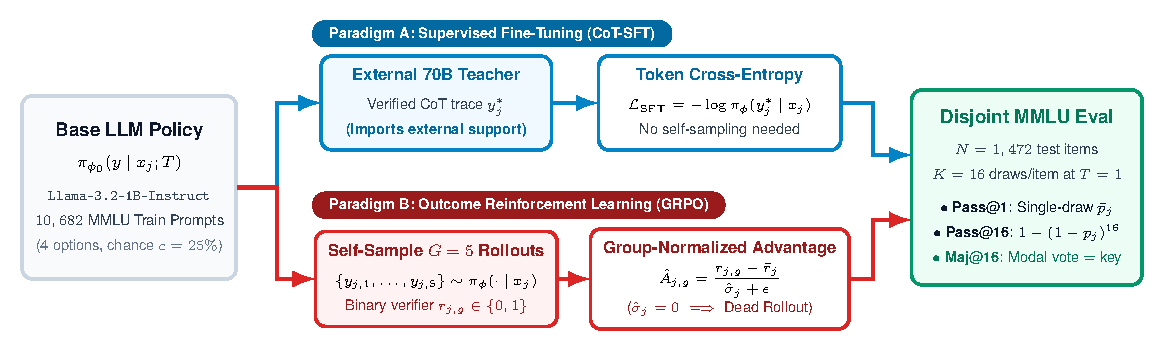
\includegraphics[height=0.50\textheight, keepaspectratio]{figures/talk_Fig00A_llm_training_tikz.pdf}
  \end{center}
  \vspace{-2.5mm}
  \begin{columns}[T, onlytextwidth]
    \begin{column}{0.32\textwidth}
      \psychbox{BlueSFT}{
        \textbf{\color{BlueSFT}1. \texttt{CoT-SFT} (External Teacher)}\\
        Minimizes token cross-entropy on verified reasoning traces $y_j^*$ from a $70\mathrm{B}$ teacher (Rafailov et al., 2023).\\
        $\bullet$ \textbf{Imports external support}: updates policy even when Base model has $p_{\mathrm{base},j}=0$.
      }
    \end{column}
    \begin{column}{0.33\textwidth}
      \psychbox{RedGRPO}{
        \textbf{\color{RedGRPO}2. \texttt{GRPO} (Self-Sampled RL)}\\
        Samples $G=5$ rollouts from current policy $\pi_\phi$, rewards binary outcome $r_{j,g}\in\{0,1\}$, normalizes within-group (Shao et al., 2024).\\
        $\bullet$ \textbf{Zero-variance trap}: if all $G$ draws fail or succeed ($\hat{\sigma}_j=0$), gradient vanishes ($\hat{A}_{j,g}=0$).
      }
    \end{column}
    \begin{column}{0.32\textwidth}
      \psychbox{GreenBase}{
        \textbf{\color{GreenBase}3. Three Disjoint Readouts}\\
        At test time ($K=16$ i.i.d.\ draws/item; Chen et al., 2021):\\
        $\bullet$ $\mathbf{Pass@1} = \hat{p}_j$: single-draw accuracy.\\
        $\bullet$ $\mathbf{Pass@16} = 1-(1-\hat{p}_j)^{16}$: multi-draw coverage.\\
        $\bullet$ $\mathbf{Maj@16} = \mathbb{I}[\arg\max_o \hat{p}_j(o) = o_j^*]$: does the \textbf{modal answer} match the key?
      }
    \end{column}
  \end{columns}
\end{frame}

% ==============================================================================
% SLIDE 3: SETUP II — HOW IRT ENTERS LLM EVALUATION & RL TRAINING
% ==============================================================================
\begin{frame}{Setup II: Where Does Offline Population 2PL IRT Enter?}{Two Entry Points: Adaptive Benchmark Evaluation vs.\ RL Advantage Critics}
  \vspace{-1.5mm}
  \begin{center}
    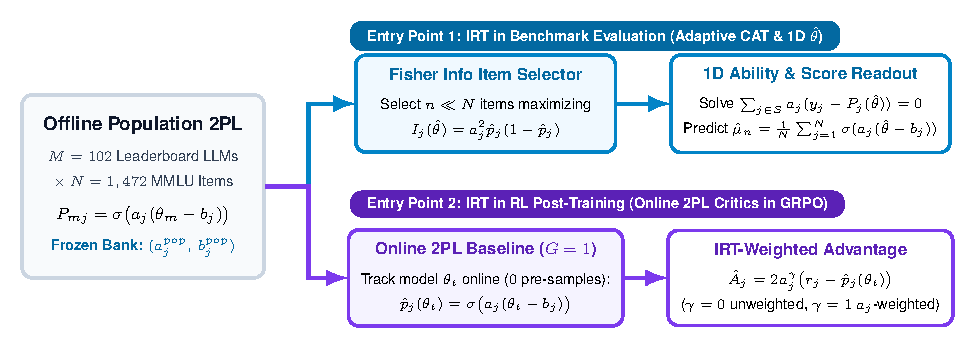
\includegraphics[height=0.50\textheight, keepaspectratio]{figures/talk_Fig00B_irt_entry_tikz.pdf}
  \end{center}
  \vspace{-2.5mm}
  \begin{columns}[T, onlytextwidth]
    \begin{column}{0.485\textwidth}
      \psychbox{BlueSFT}{
        \textbf{\color{BlueSFT}Entry Point 1: Efficient Benchmark Evaluation (Literature)}\\
        Fit a 2PL item bank $P_{mj}=\sigma(a_j(\theta_m - b_j))$ across $M=102$ Open-LLM Leaderboard models $\times$ $N=1,472$ MMLU test items (Maia Polo et al., ICML 2024; Kipnis et al., ICLR 2025).\\
        $\bullet$ \textbf{Promise}: Select $n \ll N$ high-Fisher-information items $I_j(\hat{\theta}) = a_j^2 \hat{p}_j(1-\hat{p}_j)$ via Computerized Adaptive Testing (\texttt{CAT}) to recover full-benchmark score from $32$--$128$ items.
      }
    \end{column}
    \begin{column}{0.485\textwidth}
      \psychbox{PurpleIRT}{
        \textbf{\color{PurpleIRT}Entry Point 2: Replacing Rollouts with Online 2PL Critics}\\
        Standard \texttt{GRPO} spends $G=5$ rollouts/item just to estimate baseline difficulty $\bar{r}_j$ (Hofmann et al., COLM 2025). Can frozen population $(a_j^{\mathrm{pop}}, b_j^{\mathrm{pop}})$ provide a \textbf{zero-rollout ($G=1$) baseline} and focus updates on high-$a_j$ items?\\[1mm]
        \centerline{$\hat{A}_j = 2\,a_j^\gamma\bigl(r_j - \sigma(a_j(\theta_t - b_j))\bigr), \qquad \gamma \in \{0, 1\}$}
      }
    \end{column}
  \end{columns}
\end{frame}

% ==============================================================================
% SLIDE 4: MODULE 0 — THE EMPIRICAL PUZZLE (PASS@K CROSSOVER & MAJ@16 CEILING)
% ==============================================================================
\begin{frame}{Module 0: The Empirical Puzzle --- Single-Draw Gain vs.\ Multi-Draw Collapse}{Why Aggregate Pass@1 Hides a Fundamental Support-vs.-Sharpening Divergence}
  \begin{columns}[T, onlytextwidth]
    \begin{column}{0.56\textwidth}
      \vspace{-1mm}
      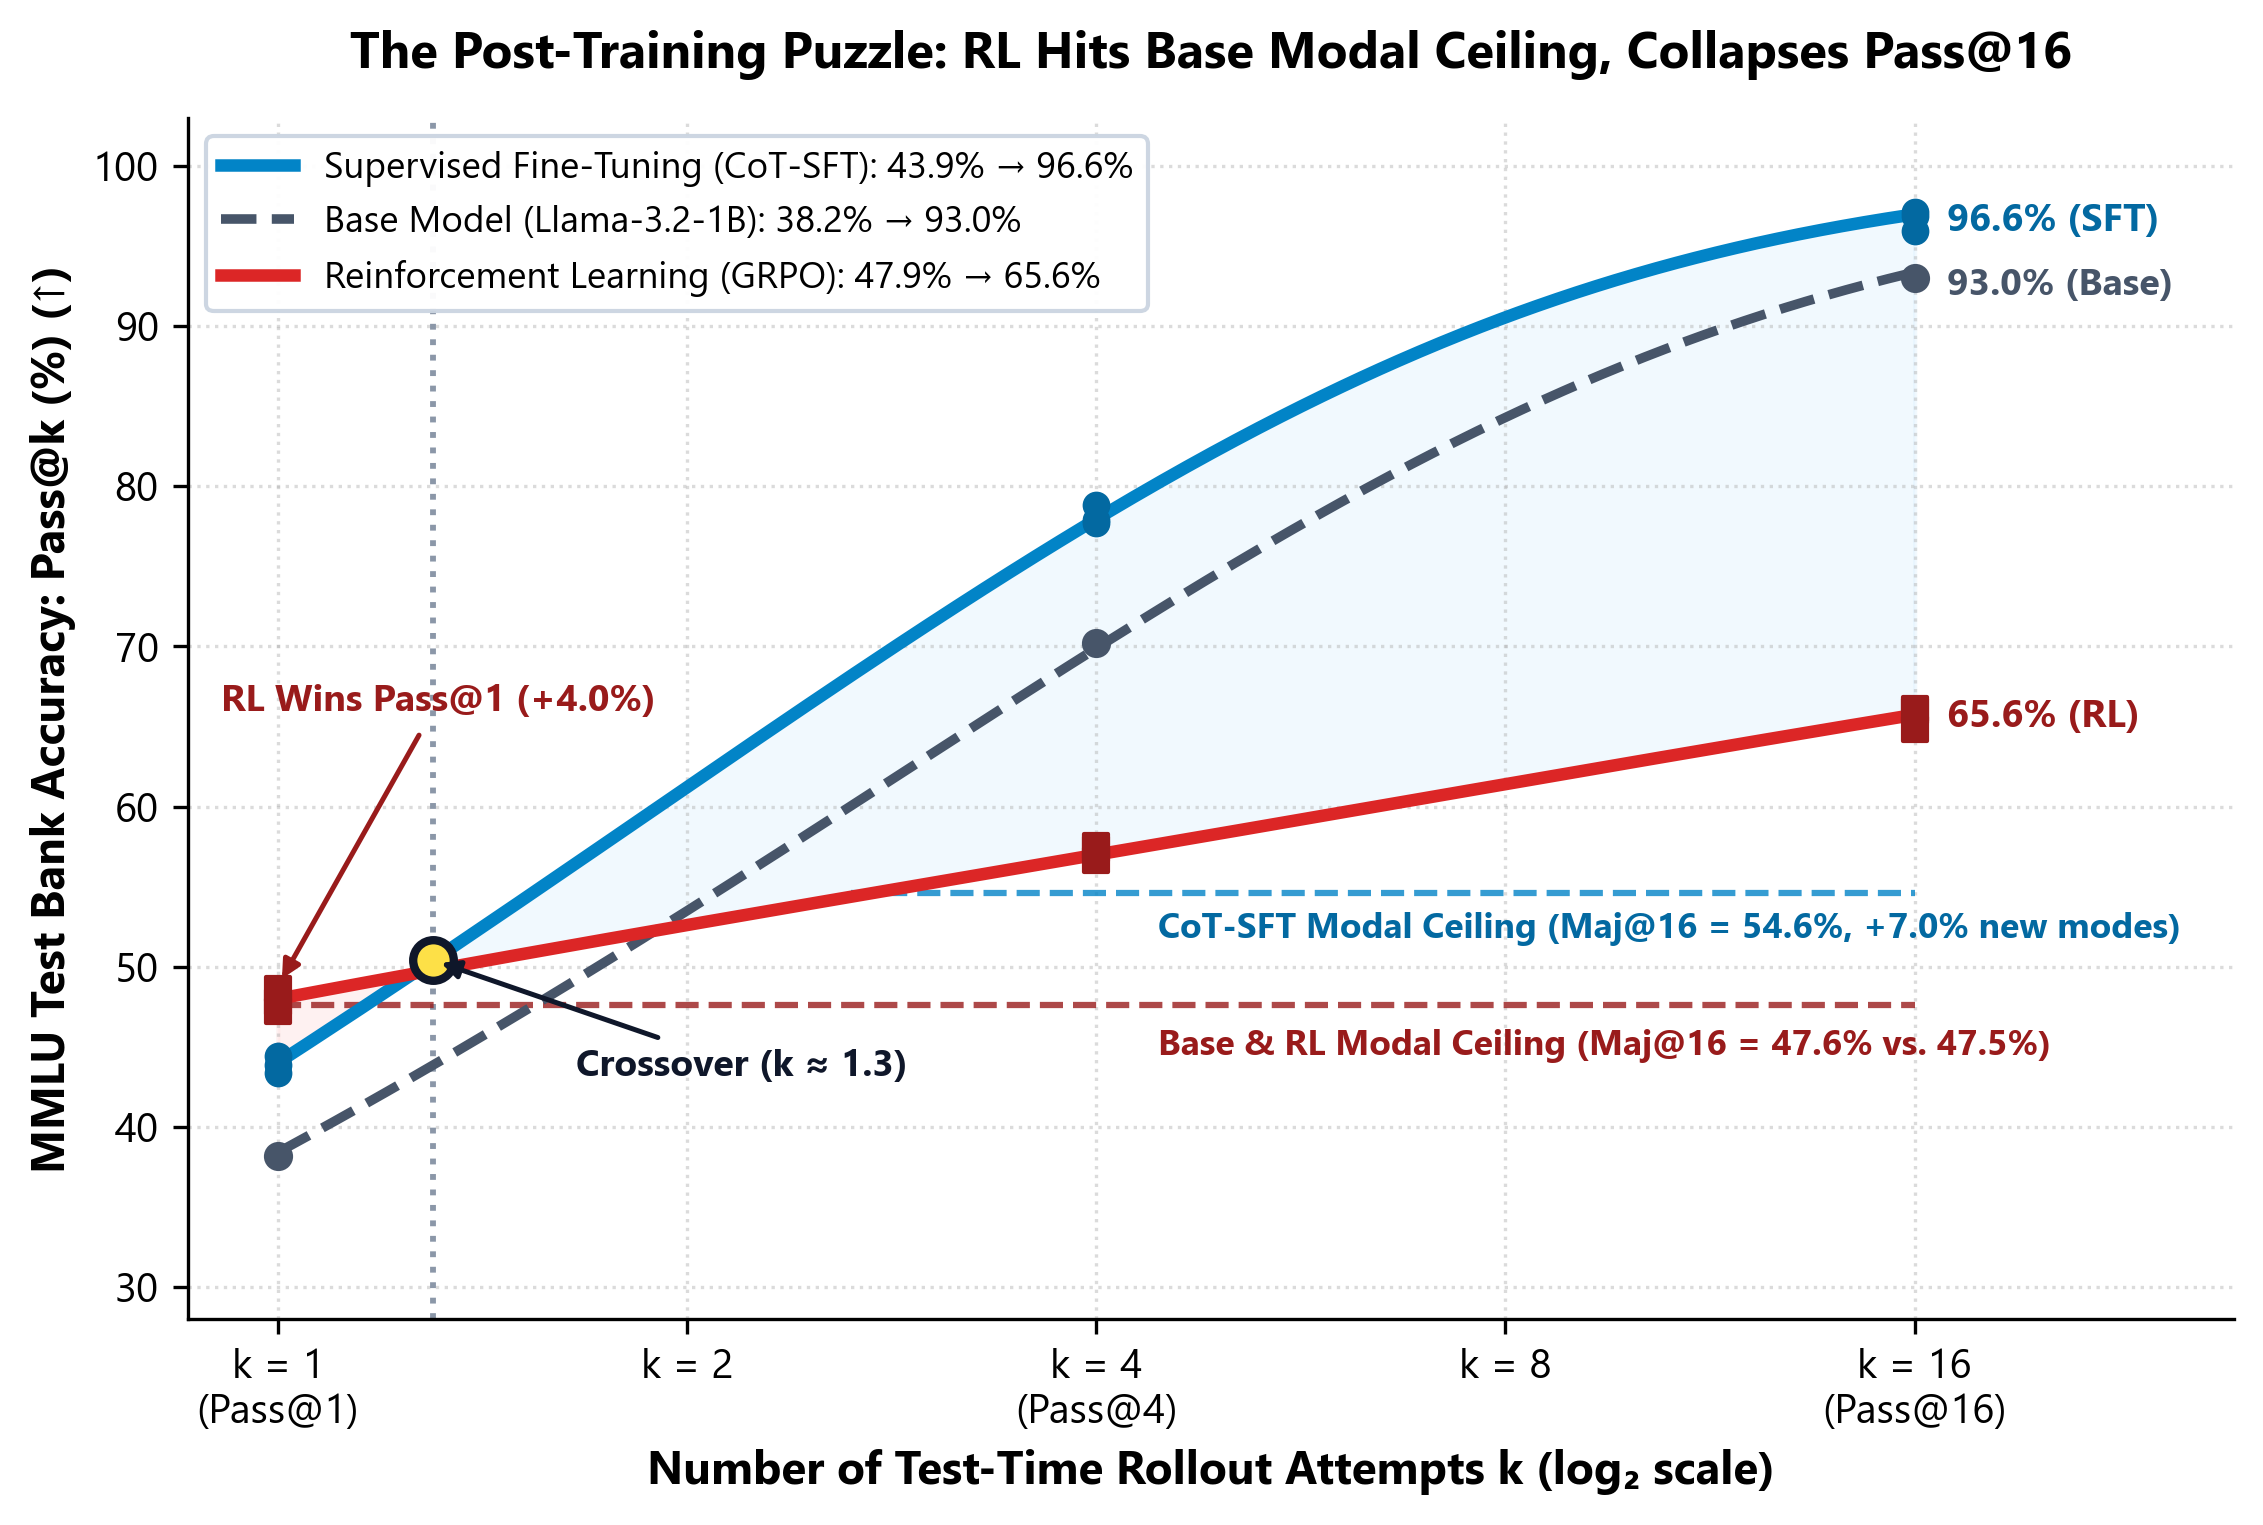
\includegraphics[width=\linewidth]{figures/talk_Fig01_puzzle_and_modal_ceiling.png}
    \end{column}
    \begin{column}{0.42\textwidth}
      \vspace{0.5mm}
      \psychbox{RedGRPO}{
        \textbf{\color{RedGRPO}What Standard ML Sees ($\mathrm{Pass@1}$ Only):}\\
        Both post-training paradigms look like clear wins over \texttt{Base} ($38.2\%$), with \texttt{GRPO} beating \texttt{CoT-SFT} by $+4.0$ pp at $k=1$:
        \begin{itemize}\setlength{\itemsep}{0.8pt}
          \item \texttt{Base (Llama-3.2-1B)}: $\mathbf{38.2\%}$
          \item \texttt{CoT-SFT}: $\mathbf{43.9\%}$ ($+5.7$ pp)
          \item \texttt{GRPO (RL)}: $\mathbf{47.9\%}$ ($+9.7$ pp)
        \end{itemize}
      }
      \vspace{1mm}
      \psychbox{BlueSFT}{
        \textbf{\color{BlueSFT}What Multi-Draw \& Modal Readouts Reveal:}\\
        \begin{itemize}\setlength{\itemsep}{1pt}
          \item \textbf{Immediate Crossover ($k \approx 1.3$)}: By $k=16$ draws, \texttt{GRPO} collapses to $\mathbf{65.6\%}$---$\mathbf{27.4\text{ pp}}$ \textbf{below} \texttt{Base} ($93.0\%$) and $\mathbf{31.0\text{ pp}}$ \textbf{below} \texttt{CoT-SFT} ($96.6\%$).
          \item \textbf{Modal-Key Ceiling ($\mathrm{Maj@16}$)}: Majority-vote accuracy is \textbf{identical} between \texttt{Base} ($\mathbf{47.6\%}$) and \texttt{GRPO} ($\mathbf{47.5\%}$), whereas \texttt{CoT-SFT} reaches $\mathbf{54.6\%}$ ($+7.0\%$ new modes).
          \item \texttt{GRPO}'s single-draw $\mathrm{Pass@1}$ ($47.9\%$) simply sharpens probability onto the Base model's pre-existing modal keys (\textbf{0\% net new modes learned}).
        \end{itemize}
      }
    \end{column}
  \end{columns}
\end{frame}

% ==============================================================================
% SLIDE 5: MODULE 1 — IRT IN EVALUATION (CONSTRUCT VALIDITY & DOMAIN DIF)
% ==============================================================================
\begin{frame}{Module 1 (Evaluation): Construct Validity \& Domain Bias in Population 2PL}{Why Adaptive CAT Hits a 2.4\% Bias Floor When Ranking Post-Trained Models}
  \vspace{-1.5mm}
  \begin{center}
    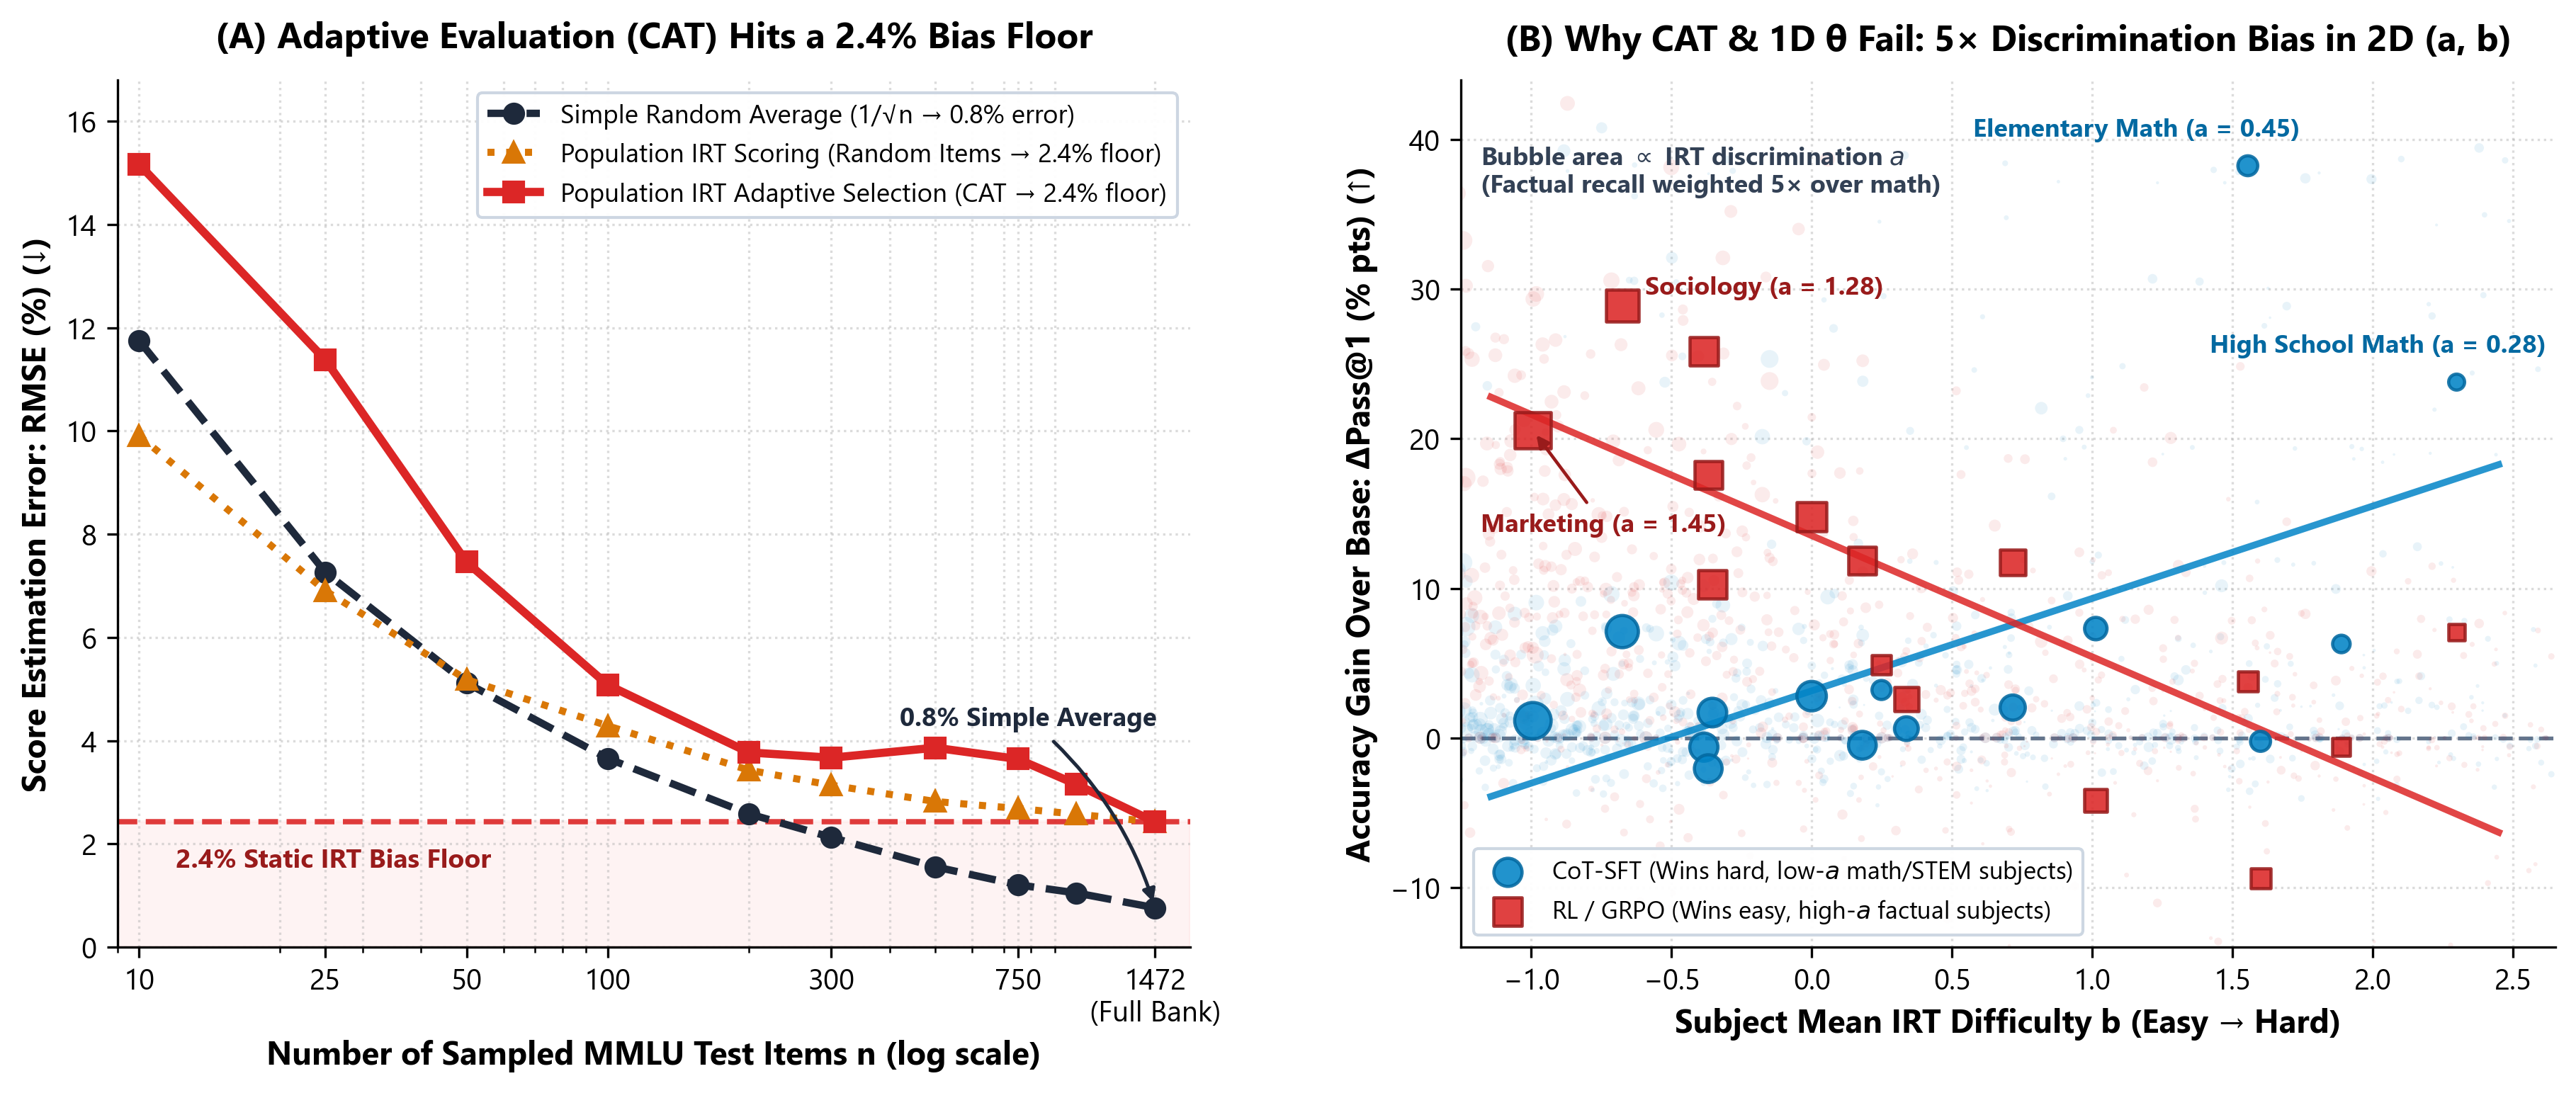
\includegraphics[height=0.51\textheight, keepaspectratio]{figures/talk_Fig02_eval_cat_and_2d_domains.png}
  \end{center}
  \vspace{-2.5mm}
  \begin{columns}[T, onlytextwidth]
    \begin{column}{0.32\textwidth}
      \psychbox{RedGRPO}{
        \textbf{\color{RedGRPO}1. Adaptive \texttt{CAT} Bias Floor ($2.4\%$)}\\
        Simple random averaging decays as $1/\sqrt{n}\to \mathbf{0.8\%}$ RMSE (Panel A), whereas population 2PL scoring and \texttt{CAT} plateau at a $\mathbf{2.4\%}$ error floor even at $n=1,472$.
      }
    \end{column}
    \begin{column}{0.34\textwidth}
      \psychbox{PurpleIRT}{
        \textbf{\color{PurpleIRT}2. Construct Validity: $5\times$ Loading Skew}\\
        In the 102-LLM bank, factual recall subjects (\emph{Marketing} $a=1.45$, \emph{Sociology} $a=1.28$) have \textbf{$5\times$ higher $a_j$} than math (\emph{HS Math} $a=0.28$). Since $I_j(\theta) \propto a_j^2$, \texttt{CAT} over-samples memory $25\times$!
      }
    \end{column}
    \begin{column}{0.31\textwidth}
      \psychbox{BlueSFT}{
        \textbf{\color{BlueSFT}3. Domain DIF Under Post-Training}\\
        \texttt{GRPO} boosts easy, high-$a$ factual domains, while \texttt{CoT-SFT} lifts hard, low-$a$ math domains (Panel B)---violating 1D measurement invariance.
      }
    \end{column}
  \end{columns}
\end{frame}

% ==============================================================================
% SLIDE 6: MODULE 2A — IRT IN RL TRAINING (4 CRITICS & EQUI-ACCURACY DIVERGENCE)
% ==============================================================================
\begin{frame}{Module 2A (RL Training): Do Population 2PL Critics Help \texttt{GRPO}?}{Aggregate Pass@1 Equivalence Masks High-k Collapse and 5/6 Equi-Accuracy Divergence}
  \vspace{-1.5mm}
  \begin{center}
    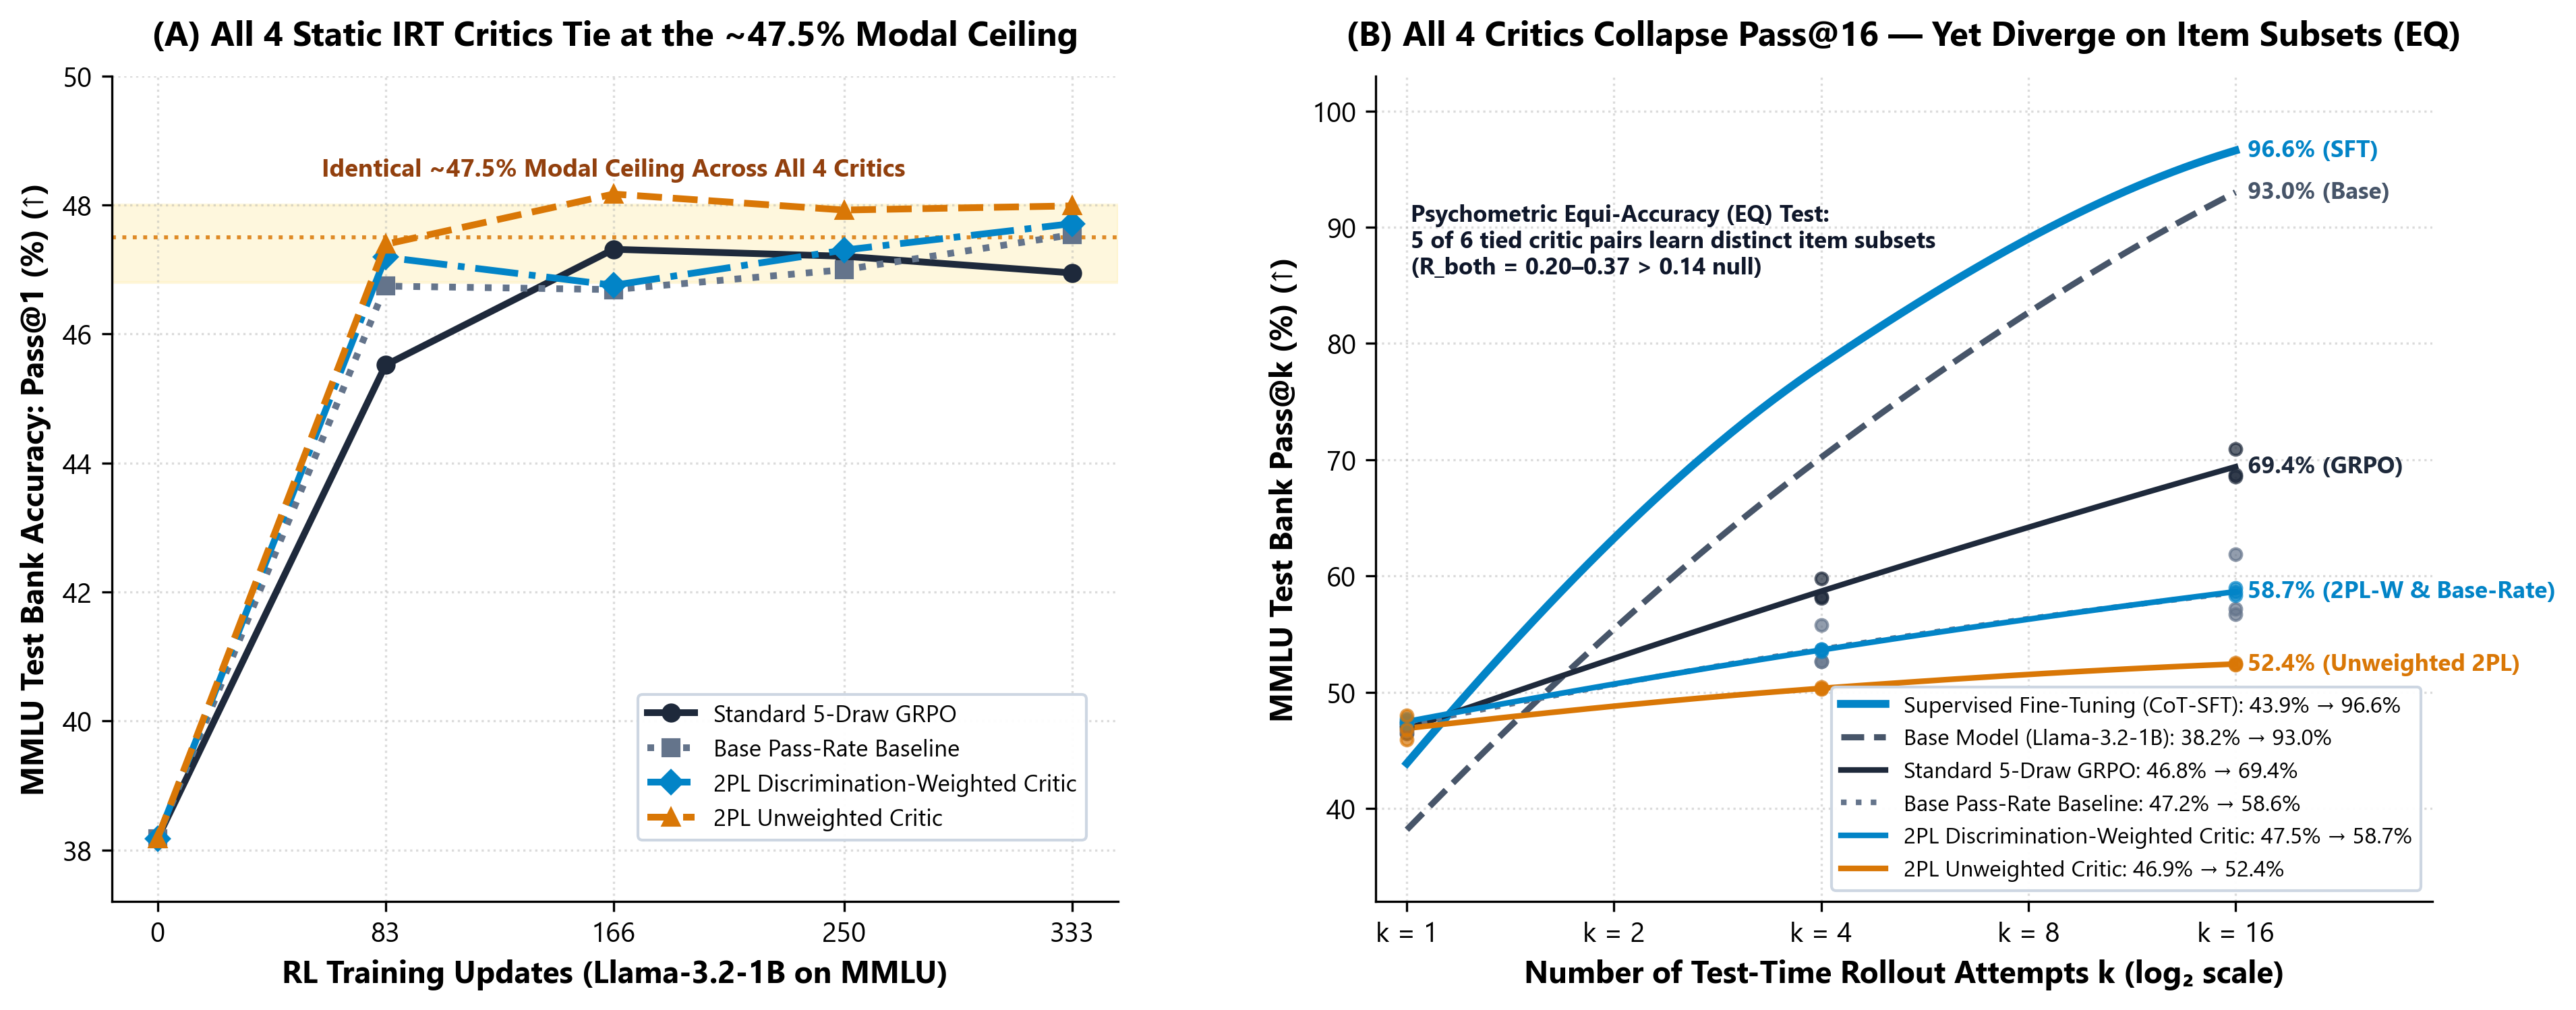
\includegraphics[height=0.51\textheight, keepaspectratio]{figures/talk_Fig03_rl_critics_and_eq_divergence.png}
  \end{center}
  \vspace{-2.5mm}
  \begin{columns}[T, onlytextwidth]
    \begin{column}{0.33\textwidth}
      \psychbox{AmberIRT}{
        \textbf{\color{AmberIRT}1. Identical $\sim 47.5\%$ $\mathrm{Pass@1}$ Ceiling}\\
        Across 333 RL updates, all 4 critics ($G=5$ \texttt{GRPO}, Base Pass-Rate, 2PL Unweighted, 2PL $a_j$-Weighted) saturate inside the exact same $\mathbf{46.8\%\text{--}47.5\%}$ modal band (Panel A).
      }
    \end{column}
    \begin{column}{0.33\textwidth}
      \psychbox{RedGRPO}{
        \textbf{\color{RedGRPO}2. Severe Multi-Draw $\mathrm{Pass@16}$ Collapse}\\
        Single-rollout critics ($G=1$) save $5\times$ sampling cost, but weighting by $a_j^{\mathrm{pop}}$ worsens multi-draw collapse at $k=16$ ($\mathbf{58.7\%}$ and $\mathbf{52.4\%}$ vs.\ $93.0\%$ Base, Panel B).
      }
    \end{column}
    \begin{column}{0.31\textwidth}
      \psychbox{PurpleIRT}{
        \textbf{\color{PurpleIRT}3. Equi-Accuracy (\texttt{EQ}) Divergence}\\
        Conditioning on tied $\mathrm{Pass@1}$, \textbf{5 of 6 critic pairs} solve significantly different item subsets ($R_{\mathrm{both}} = 0.20\text{--}0.37 > 0.14$ null).
      }
    \end{column}
  \end{columns}
\end{frame}

% ==============================================================================
% SLIDE 7: MODULE 2B — COORDINATE FRAME & FIRST-ORDER TRAJECTORY ORTHOGONALITY
% ==============================================================================
\begin{frame}{Module 2B (Coordinate Frame): Why Population $(a_j^{\mathrm{pop}}, b_j^{\mathrm{pop}})$ Fails in RL}{Between-Respondent Calibration vs.\ Within-Model Repeated-Trial Calibration}
  \begin{columns}[T, onlytextwidth]
    \begin{column}{0.55\textwidth}
      \vspace{-1.5mm}
      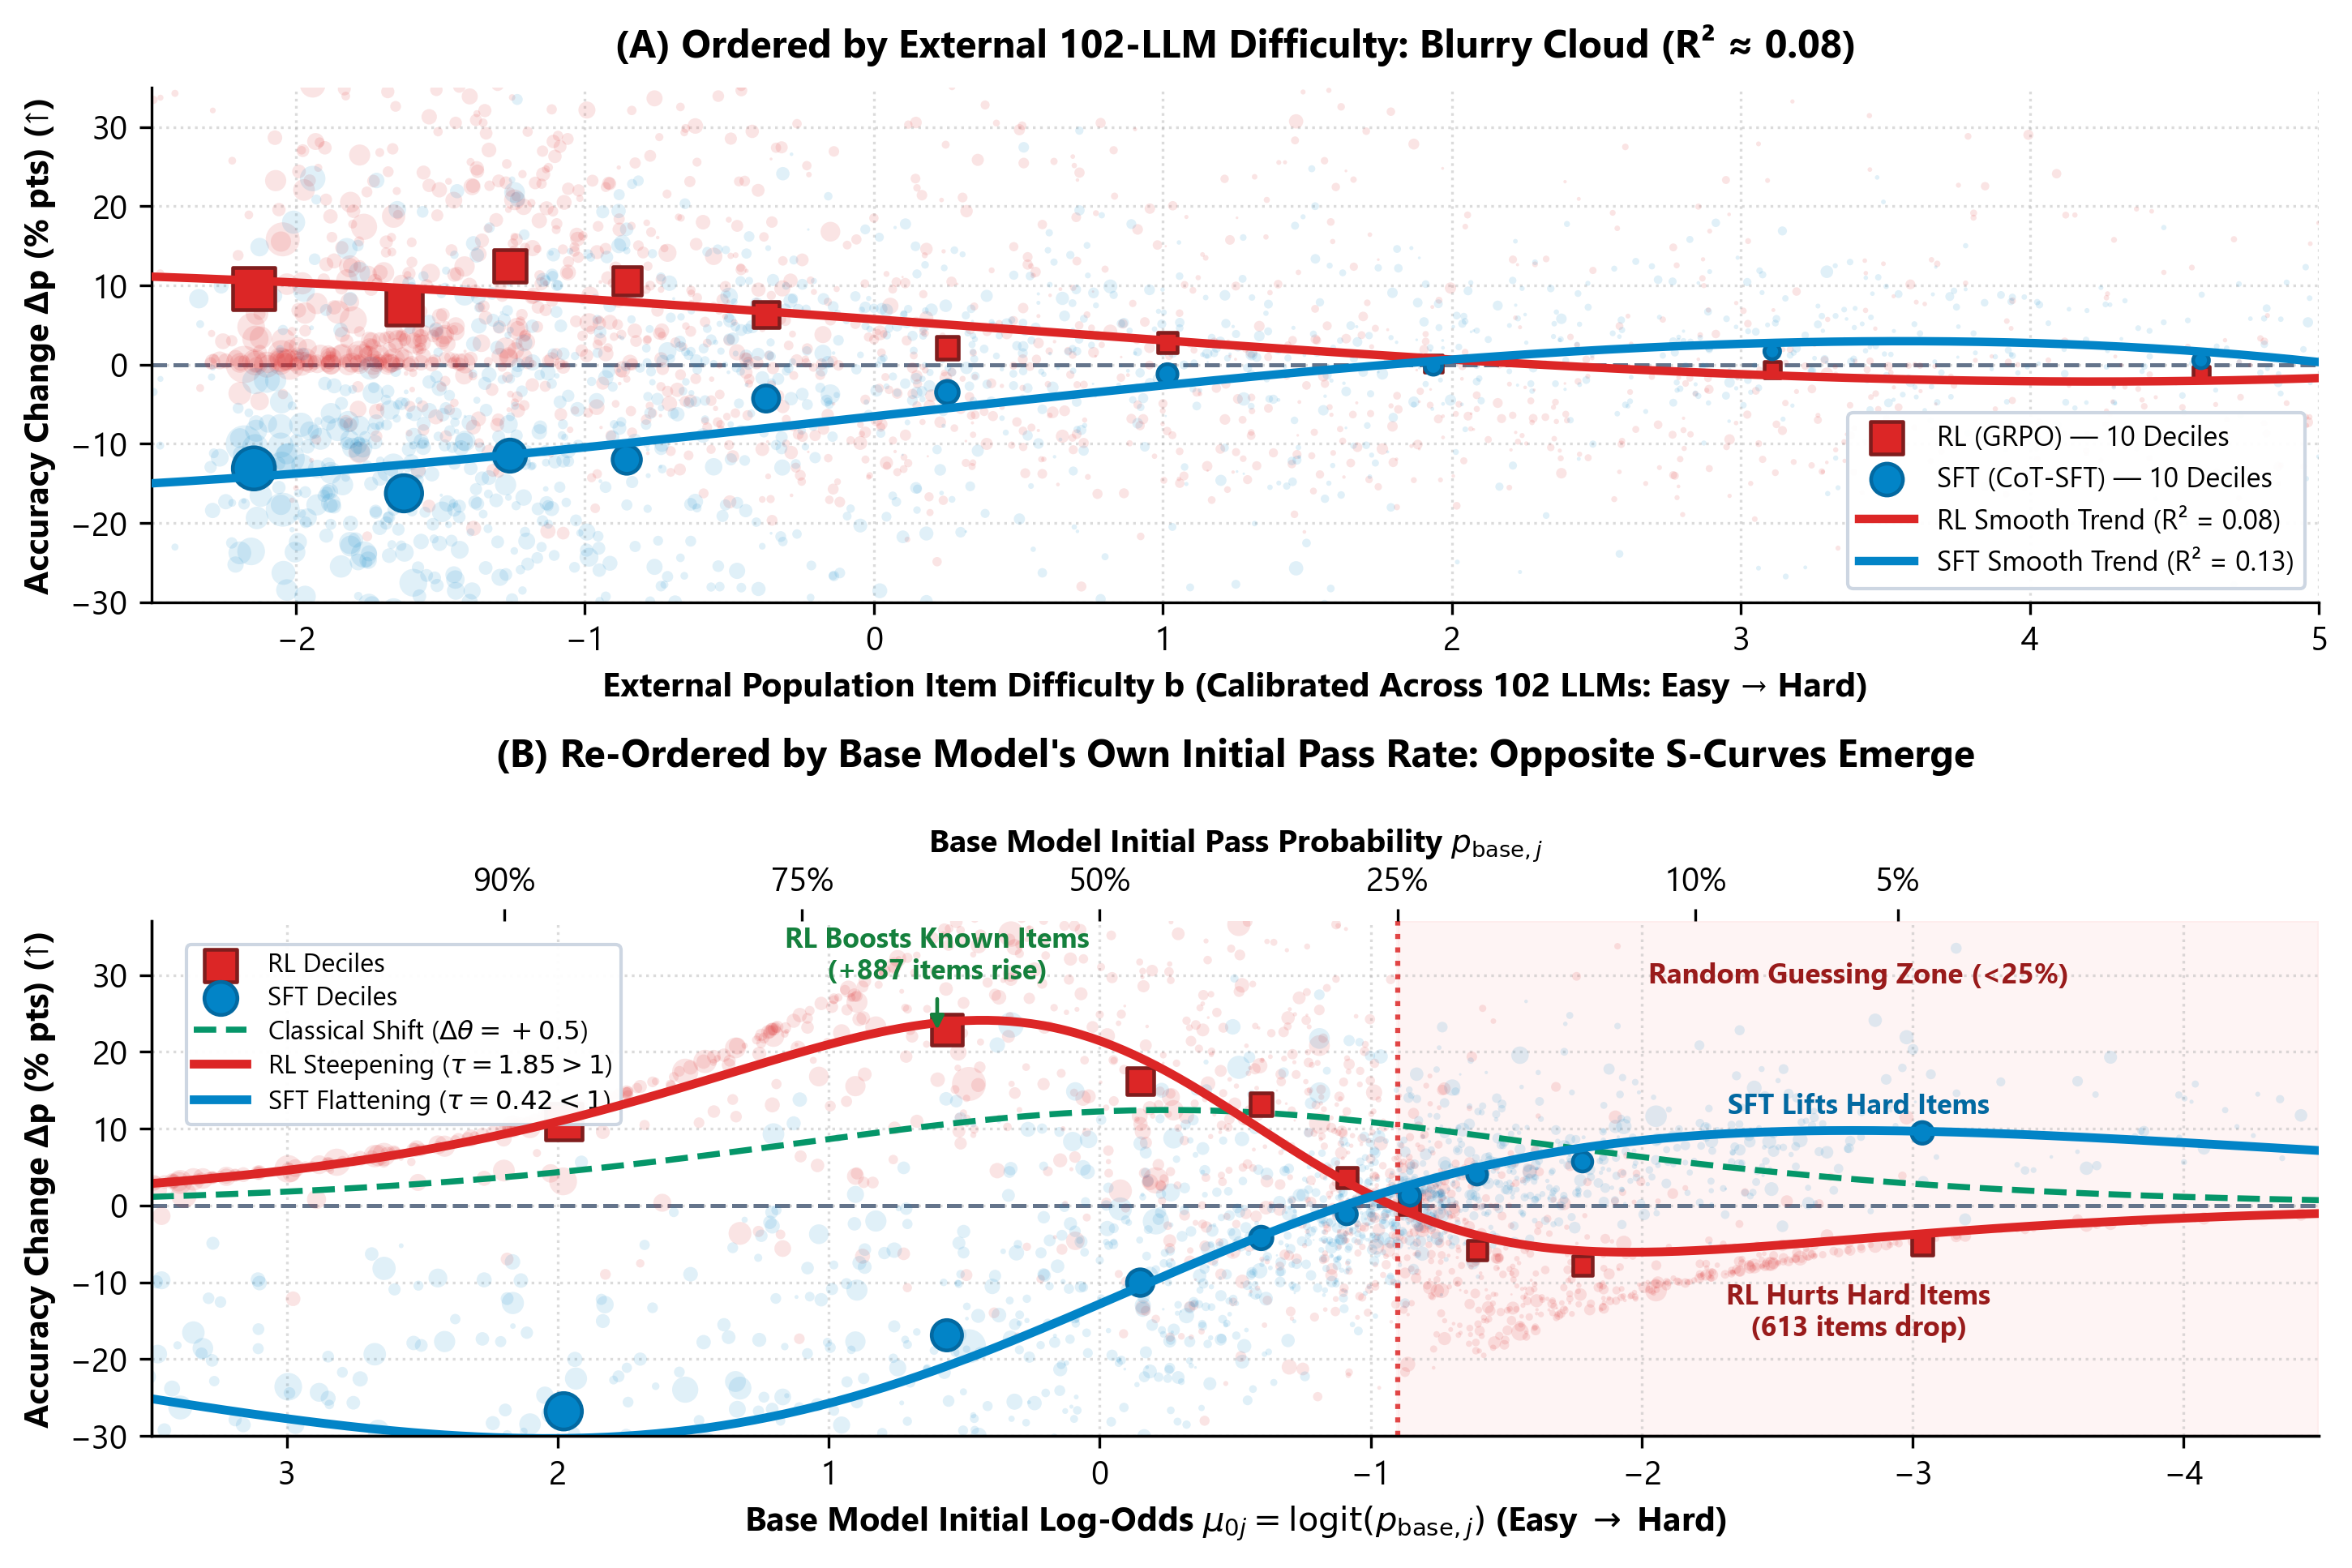
\includegraphics[width=\linewidth]{figures/talk_Fig04_coordinate_translation_stacked.png}
    \end{column}
    \begin{column}{0.43\textwidth}
      \vspace{0.2mm}
      \psychbox{RedGRPO}{
        \textbf{\color{RedGRPO}1. Between-Respondent Coordinate Mismatch}\\
        Ordering items by \textbf{external 102-LLM difficulty $b_j^{\mathrm{pop}}$} yields a blurry cloud ($R^2 = 0.08$, Panel A). $b_j^{\mathrm{pop}}$ captures cross-architecture scale differences across 102 models, not difficulty for our single 1B policy.
      }
      \vspace{1mm}
      \psychbox{PurpleIRT}{
        \textbf{\color{PurpleIRT}2. First-Order Trajectory Jacobian Orthogonality}\\
        Linearizing the policy logit change $\Delta z_j$ along update $\Delta\phi$:\\[0.8mm]
        {\centering $\Delta z_j \approx J_j \Delta\phi = \alpha_{\parallel} a_j^{\mathrm{pop}} + J_j u_{\perp}$\par}\vspace{0.8mm}
        The within-model update subspace $J_j u_{\perp}$ is \textbf{orthogonal to population discrimination}:\\[0.8mm]
        {\centering $\mathbf{\mathrm{corr}(J_j u_{\perp},\, a_j^{\mathrm{pop}}) = 0.072}, \quad \mathrm{corr}(\Delta p_j^{\mathrm{RL}},\, a_j^{\mathrm{pop}}) = +0.025$\par}
      }
      \vspace{1mm}
      \psychbox{BlueSFT}{
        \textbf{\color{BlueSFT}3. Within-Respondent Calibration $\mu_{0j} = \mathrm{logit}(p_{\mathrm{base},j})$}\\
        Re-ordering by the Base model's own $K=16$ repeated-trial log-odds $\mu_{0j}$ snaps the cloud into \textbf{two opposite S-curves crossing at $c = 1/K = 25\%$} (Panel B)!
      }
    \end{column}
  \end{columns}
\end{frame}

% ==============================================================================
% SLIDE 8: MODULE 3 — PERSON RESPONSE FUNCTION (PRF) SLOPE & 3PL DISTRACTORS
% ==============================================================================
\begin{frame}{Module 3 (Psychometric Mechanism): PRF Slope Rotation \& 3PL Distractor Lock-In}{Translating Temperature Scaling and RL Sharpening into Item Response Theory}
  \begin{columns}[T, onlytextwidth]
    \begin{column}{0.54\textwidth}
      \vspace{-1mm}
      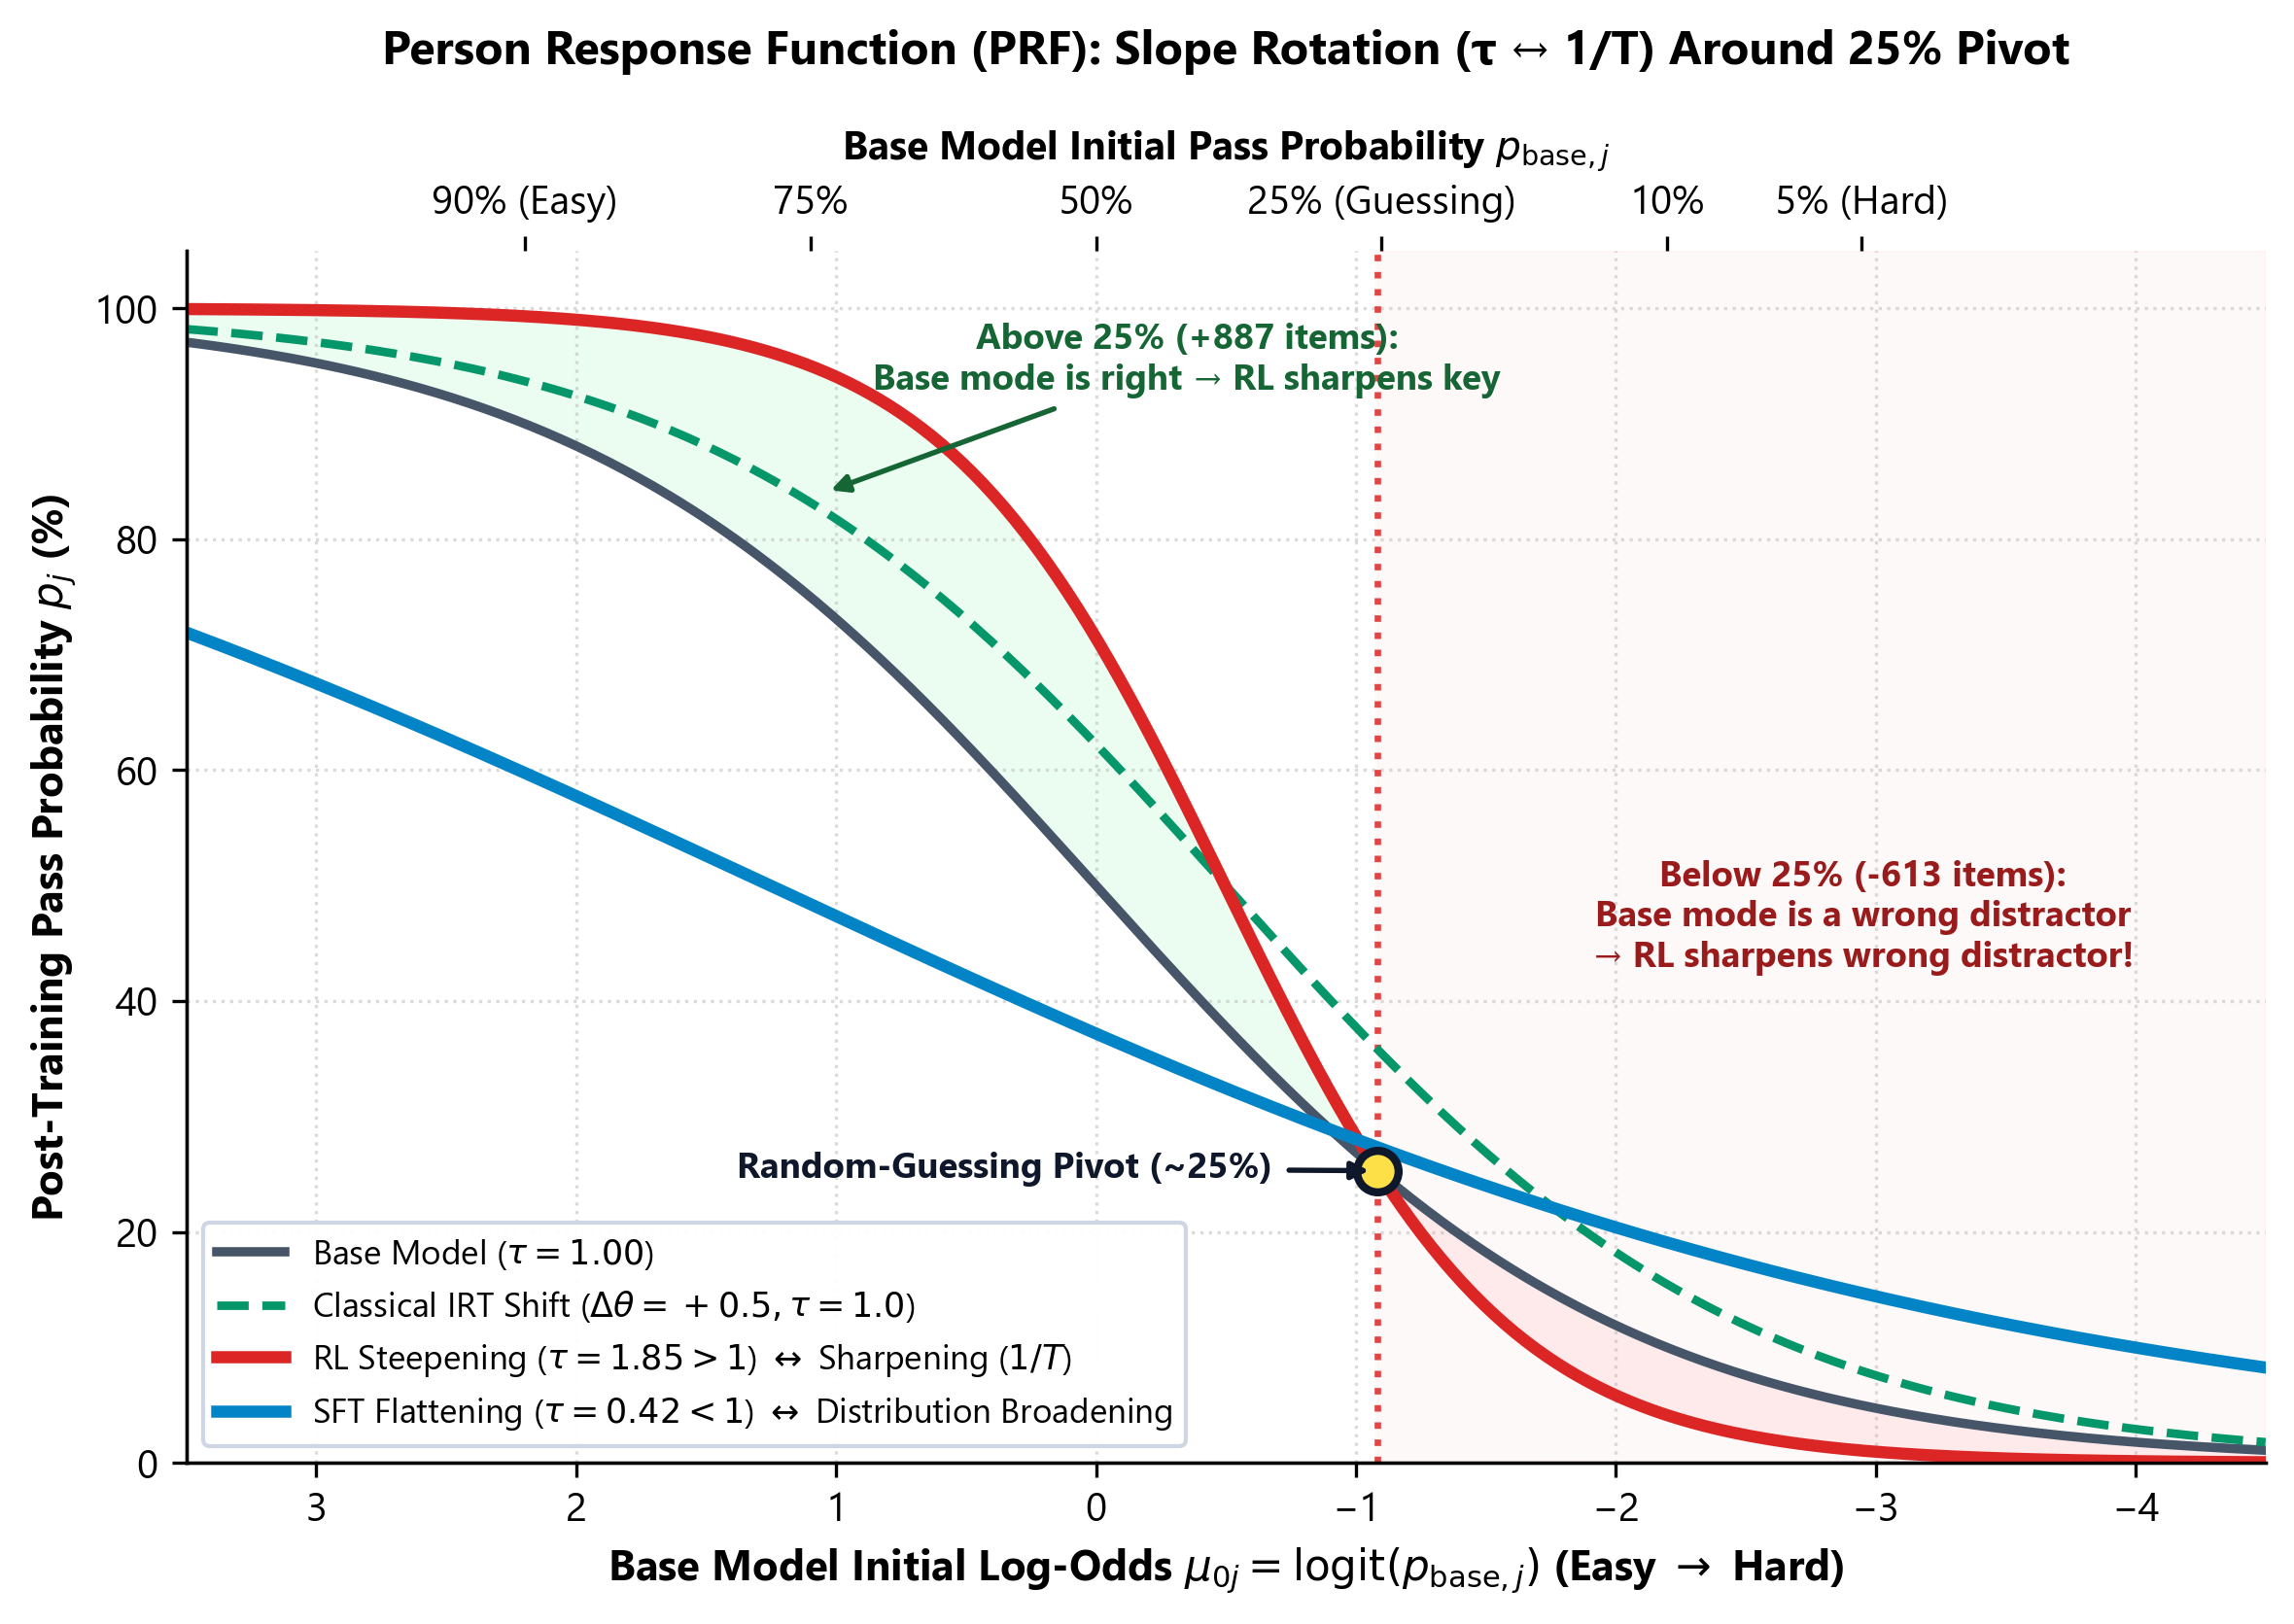
\includegraphics[width=\linewidth]{figures/talk_Fig05_prf_slope_and_distractor_pivot.png}
    \end{column}
    \begin{column}{0.44\textwidth}
      \vspace{0.2mm}
      \psychbox{PurpleIRT}{
        \textbf{\color{PurpleIRT}1. Person Response Function (PRF) Parameterization}\\
        In psychometrics (Trabasso, 1973; Embretson \& Reise, 2000), a respondent's operating curve across within-person easiness $\mu_{0j}$ is a \textbf{Person Response Function}:\\[0.8mm]
        {\centering $p_{s,j} = \sigma\!\bigl(\alpha_s + \tau_s(\mu_{0j} - \mu_c)\bigr), \quad \mu_c = \mathrm{logit}(0.25) = -1.10$\par}\vspace{0.8mm}
        $\bullet$ \textbf{Intercept $\alpha_s$}: Horizontal knowledge shift (new support).\\
        $\bullet$ \textbf{PRF Slope $\tau_s \leftrightarrow 1/T$}: Inverse decoding temperature!
      }
      \vspace{1mm}
      \psychbox{RedGRPO}{
        \textbf{\color{RedGRPO}2. The 3PL Distractor Trap Below $c = 25\%$}\\
        Why does \texttt{GRPO} ($\tau_{\mathrm{RL}} = 1.85 > 1$) \textbf{suppress} accuracy below the Base curve on $613$ items with $p_{\mathrm{base},j} < 25\%$?\\
        In a 4-choice item (Thissen \& Steinberg, 1984), $p_{\mathrm{base},j} < 0.25$ implies a \textbf{plausible wrong distractor $d^*$} holds the mode ($p_{\mathrm{base}}(d^*) > 0.25$). Outcome RL \textbf{sharpens the wrong modal distractor} ($p_{\mathrm{RL}}(o^*) \to 0$), destroying $\mathrm{Pass@16}$!\\
        Conversely, \texttt{CoT-SFT} ($\tau_{\mathrm{SFT}} = 0.42 < 1$) lifts hard items above chance.
      }
    \end{column}
  \end{columns}
\end{frame}

% ==============================================================================
% SLIDE 9: MODULE 4 — LOCAL INDEPENDENCE VIOLATION & FORMAT DIF
% ==============================================================================
\begin{frame}{Module 4 (Diagnostic Added Value): Local Independence \& Format DIF}{Two Structural Pathologies Invisible to Aggregate Benchmark Scores}
  \vspace{-1.5mm}
  \begin{center}
    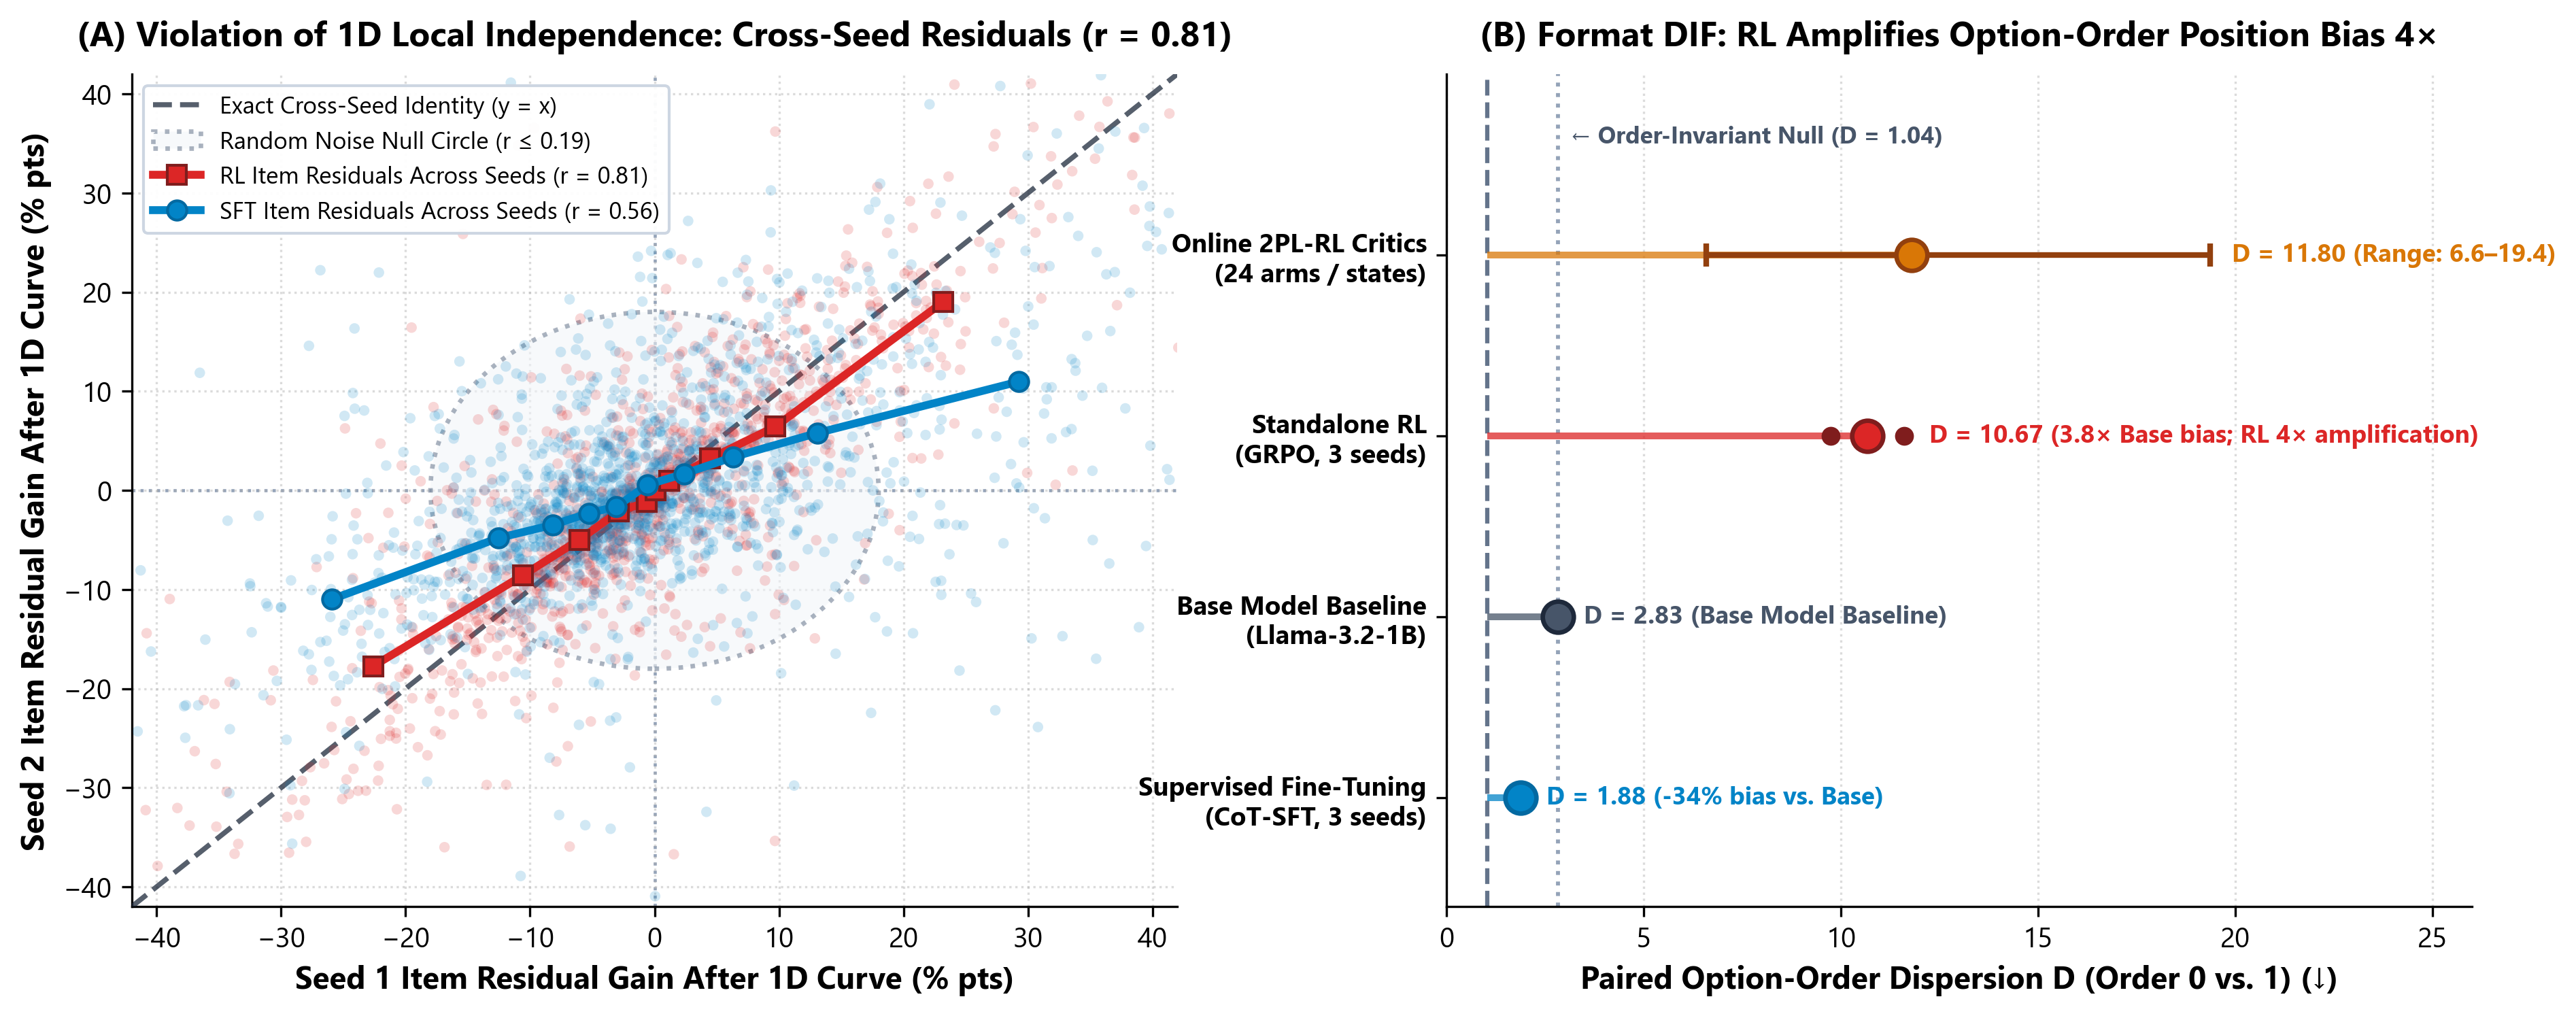
\includegraphics[height=0.51\textheight, keepaspectratio]{figures/talk_Fig06_local_independence_and_order_dif.png}
  \end{center}
  \vspace{-2.5mm}
  \begin{columns}[T, onlytextwidth]
    \begin{column}{0.485\textwidth}
      \psychbox{PurpleIRT}{
        \textbf{\color{PurpleIRT}1. Violation of Conditional Local Independence ($r = 0.81$)}\\
        Under a 1D latent update, item residuals $e_j = \Delta p_j - \widehat{\Delta p}_j(\mu_{0j})$ across independent random training seeds should be uncorrelated noise ($r \le 0.19$ null circle, Panel A). Instead, cross-seed residuals correlate at $\mathbf{r = 0.81}$ in RL ($r = 0.56$ in SFT): over \textbf{$80\%$ of residual item variance is deterministic multi-dimensional structure} locked to the Base initialization.
      }
    \end{column}
    \begin{column}{0.485\textwidth}
      \psychbox{RedGRPO}{
        \textbf{\color{RedGRPO}2. Format DIF: $4\times$ Option-Order Position Bias ($D = 10.67$)}\\
        Swapping option order (\texttt{Order 0 vs.\ 1}) tests format invariance via paired dispersion $D$ (Panel B). While \texttt{CoT-SFT} \emph{reduces} position bias by $-34\%$ ($D = \mathbf{1.88}$ vs.\ $\mathbf{2.83}$ Base), \texttt{GRPO} and Online 2PL-RL critics \textbf{amplify position bias $4\times$} ($D = \mathbf{10.67}$ and $\mathbf{11.80}$): when $\tau > 1$ sharpens low-certainty items, it locks onto letter-position heuristics!
      }
    \end{column}
  \end{columns}
\end{frame}

% ==============================================================================
% SLIDE 10: MODULE 5 — TESTING THE PSYCHOMETRIC PREDICTIONS
% ==============================================================================
\begin{frame}{Module 5: Testing Three Falsifiable Predictions of the Psychometric Model}{Temperature Isomorphism, Two-Stage Composition, and 1PL Fisher Information Filtering}
  \vspace{-1.5mm}
  \begin{center}
    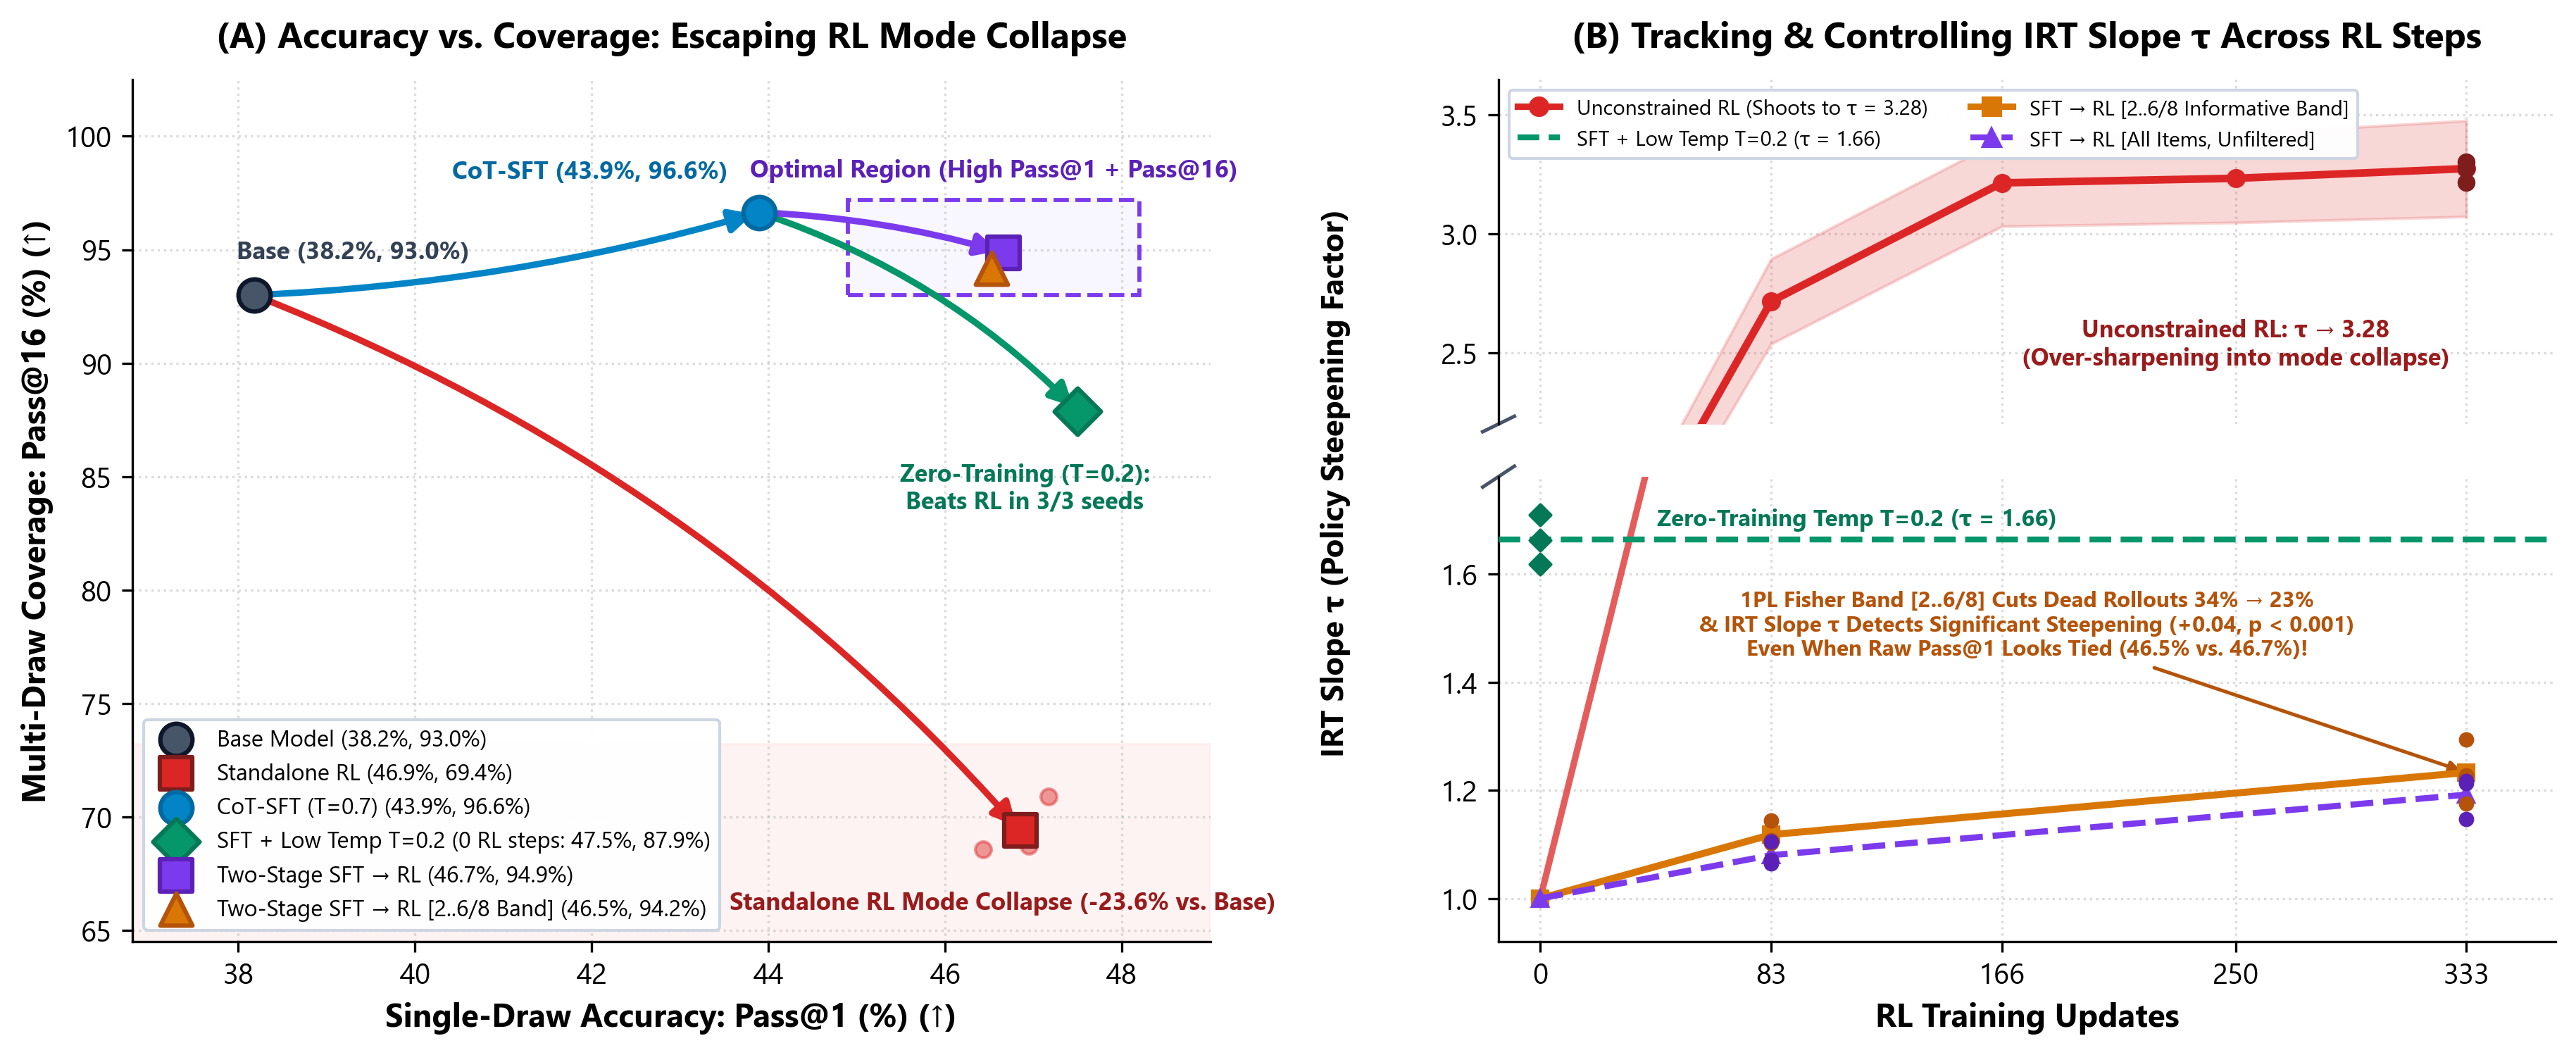
\includegraphics[height=0.51\textheight, keepaspectratio]{figures/talk_Fig07_predictions_and_fisher_band.png}
  \end{center}
  \vspace{-2.5mm}
  \begin{columns}[T, onlytextwidth]
    \begin{column}{0.32\textwidth}
      \psychbox{GreenBase}{
        \textbf{\color{GreenBase}1. Temp Isomorphism ($\tau \leftrightarrow 1/T$)}\\
        Decoding \texttt{CoT-SFT} at $\mathbf{T=0.2}$ (\textbf{0 RL steps}, $\tau=1.66$) jumps from $43.9\% \to \mathbf{47.5\%}$ $\mathrm{Pass@1}$ while retaining $\mathbf{87.9\%}$ $\mathrm{Pass@16}$---beating standalone RL in $3/3$ seeds (Panel A)!
      }
    \end{column}
    \begin{column}{0.33\textwidth}
      \psychbox{PurpleIRT}{
        \textbf{\color{PurpleIRT}2. Two-Stage \texttt{CoT-SFT $\to$ RL}}\\
        First shifting support via \texttt{CoT-SFT} ($\alpha>0$) and then applying controlled RL reaches the Pareto box ($\mathbf{46.7\%}$ $\mathrm{Pass@1}$, $\mathbf{94.9\%}$ $\mathrm{Pass@16}$) without mode collapse ($\tau = 1.19$ vs.\ $3.28$).
      }
    \end{column}
    \begin{column}{0.32\textwidth}
      \psychbox{AmberIRT}{
        \textbf{\color{AmberIRT}3. 1PL Fisher Band $[2..6/8]$}\\
        Selecting active items with within-model Fisher info $I_j^{\mathrm{within}} = p_j(1-p_j) > 0$ cuts dead rollouts $\mathbf{34\%\to 23\%}$ and steepens $\tau_t$ ($\mathbf{+0.04, p<0.001}$, Panel B) even when $\mathrm{Pass@1}$ ties!
      }
    \end{column}
  \end{columns}
\end{frame}

% ==============================================================================
% SLIDE 11: SYNTHESIS — WHAT ML MISSES VS. WHAT PSYCHOMETRICS REVEALS
% ==============================================================================
\begin{frame}{Synthesis: What Standard ML Metrics Miss vs.\ What Psychometrics Reveals}{Five Structural Insights Across LLM Benchmark Evaluation and Post-Training}
  \vspace{-2.5mm}
  \renewcommand{\arraystretch}{1.06}
  \setlength{\tabcolsep}{3.5pt}
  \tiny
  \begin{tabular}{>{\bfseries\color{NavyHeader}\raggedright\arraybackslash}p{2.25cm} >{\raggedright\arraybackslash}p{3.35cm} >{\color{PurpleIRT}\bfseries\raggedright\arraybackslash}p{3.15cm} >{\raggedright\arraybackslash}p{5.15cm}}
    \toprule
    \textbf{Stage / Arena} & \textbf{\color{RedGRPO}Superficial ML Practice (CTT)} & \textbf{Psychometric / IRT Lens} & \textbf{\color{BlueSFT}New Structural Finding in Our Study} \\
    \midrule
    1. Adaptive Eval (\texttt{CAT} / 1D $\hat{\theta}$) &
    Compress 100+ LLMs into a 1D score $\hat{\theta}$; claim $32$--$100$ items suffice. &
    Construct Validity, Factor Loading $(a_s, b_s)$ \& Domain DIF &
    Population $a_j^{\mathrm{pop}}$ loads \textbf{$5\times$ heavier on factual recall} ($a=1.45$) than math ($a=0.28$), causing a $\mathbf{2.4\%}$ \texttt{CAT} bias floor under post-training. \\
    \rowcolor{LightBg}
    2. RL Critics \& Item Weighting &
    Plug static leaderboard $(a_j^{\mathrm{pop}}, b_j^{\mathrm{pop}})$ into RL advantage $\hat{A}_j$; check only $\mathrm{Pass@1}$. &
    Between- vs.\ Within-Person Frame \& Equi-Accuracy (\texttt{EQ}) &
    All 4 critics tie at $\sim 47.5\%$ $\mathrm{Pass@1}$ ($\mathrm{corr}(J_j u_\perp, a_j^{\mathrm{pop}})=0.072$), yet diverge on \textbf{5/6 \texttt{EQ} item subsets} and collapse at $\mathrm{Pass@16}$. \\
    3. SFT vs.\ RL Post-Training &
    Compare aggregate $\mathrm{Pass@1}$ ($43.9\%$ vs.\ $47.9\%$) and treat RL as new reasoning. &
    Person Response Function (PRF) Slope $\tau_s$ \& 3PL Distractors &
    \texttt{GRPO} rotates PRF slope ($\tau=1.85 \leftrightarrow 1/T$) around $c=25\%$, learning \textbf{0\% net new modes} ($\mathrm{Maj@16}=47.5\%$) and locking in wrong distractors below $25\%$. \\
    \rowcolor{LightBg}
    4. Residual \& Format Audits &
    Ignore item residuals and average over prompt formatting. &
    Local Independence ($r_{e,e'}$) \& Option-Order Format DIF ($D$) &
    Cross-seed updates violate 1D local independence ($\mathbf{r=0.81}$), and \texttt{GRPO} amplifies option-order bias \textbf{$4\times$} ($D=\mathbf{10.67}$ vs.\ $1.88$ in SFT). \\
    5. Curriculum \& Control &
    Heuristic rollout filtering monitored only via aggregate $\mathrm{Pass@1}$. &
    Within-Model 1PL Fisher Info $I_j = p_j(1-p_j)$ \& $(\alpha_t, \tau_t)$ Tracker &
    Decoding \texttt{CoT-SFT} at $T=0.2$ reaches $\mathbf{47.5\%}$ with 0 RL steps; Fisher band $[2..6/8]$ cuts dead rollouts $34\%\to 23\%$ and steepens $\tau_t$ ($p<0.001$). \\
    \bottomrule
  \end{tabular}

  \vspace{1.5mm}
  \takeawaybox{
    \textbf{\color{NavyHeader}Core Takeaway for Psychometricians \& ML Researchers:} Classical IRT parameters $(a_j^{\mathrm{pop}}, b_j^{\mathrm{pop}})$ fail as \emph{static training weights} not because IRT is irrelevant to LLMs, but because \textbf{cross-population differences are orthogonal to within-model learning dynamics}. Once formulated in the \textbf{within-respondent frame}, psychometric theory provides exact, falsifiable diagnostics that aggregate ML metrics miss.
  }
\end{frame}

% ==============================================================================
% SLIDE 12: OPEN DISCUSSION & NEXT STEPS FOR OUR GROUP
% ==============================================================================
\begin{frame}{Open Discussion: Where Should Our Psychometrics $\times$ LLM Agenda Go Next?}{Three Concrete Questions for Group Feedback}
  \vspace{0.5mm}
  \begin{columns}[T, onlytextwidth]
    \begin{column}{0.32\textwidth}
      \psychbox{BlueSFT}{
        \textbf{\color{BlueSFT}\small Q1. Multi-Dimensional CAT \& DIF-Aware Evaluation}\\[1.5mm]
        Since unidimensional $\theta_{\mathrm{pop}}$ over-selects high-$a_j$ factual memorization items ($5\times$ skew) and breaks measurement invariance across \texttt{Base}, \texttt{CoT-SFT}, and \texttt{GRPO}:\\[1.5mm]
        $\bullet$ Should our next evaluation step be a \textbf{2D / Bi-Factor Adaptive Test} $(\theta_{\mathrm{memory}}, \theta_{\mathrm{reasoning}})$ with domain-stratified Fisher information constraints?\\[1mm]
        $\bullet$ Can we standardize \textbf{Option-Order Format DIF ($D$)} as a diagnostic for RL over-sharpening?
      }
    \end{column}
    \begin{column}{0.32\textwidth}
      \psychbox{PurpleIRT}{
        \textbf{\color{PurpleIRT}\small Q2. Nominal Response / 3PL Models Below $c = 25\%$}\\[1.5mm]
        Our strongest mechanistic finding is the \textbf{polarity flip at the $c = 1/K = 25\%$ guessing threshold}, where outcome RL amplifies attractive wrong distractors:\\[1.5mm]
        $\bullet$ Can we model the full 4-option probability vector $(p_A, p_B, p_C, p_D)$ using \textbf{Bock's Nominal Response Model (NRM)} or a \textbf{3PL distractor-repulsion penalty}?\\[1mm]
        $\bullet$ How should we regularize confidence sharpening when $p_{\mathrm{base},j} \le 1/K$?
      }
    \end{column}
    \begin{column}{0.32\textwidth}
      \psychbox{TealTwoStage}{
        \textbf{\color{TealTwoStage}\small Q3. Trajectory-Calibrated Longitudinal Item Banks}\\[1.5mm]
        Cross-seed residuals show that $81\%$ of item learning structure is reproducible across training runs ($r = 0.81$), just invisible to static leaderboard calibration:\\[1.5mm]
        $\bullet$ Instead of calibrating $(a_j, b_j)$ across 102 heterogeneous leaderboard models, can we calibrate a \textbf{Longitudinal / State-Space Growth Curve Model} across checkpoints $\phi_0 \to \phi_t$?\\[1mm]
        $\bullet$ How few anchor items suffice to track $(\alpha_t, \tau_t)$ online?
      }
    \end{column}
  \end{columns}

  \vspace{2mm}
  \begin{center}
    
\begin{tikzpicture}
      \node[draw=NavyHeader, fill=NavyHeader, text=white, rounded corners=4pt, inner xsep=12pt, inner ysep=4.5pt, font=\footnotesize\bfseries]
        {Thank You! \quad Floor Open for Discussion on Psychometric Diagnostics for LLM Evaluation \& Training};
    \end{tikzpicture}
  \end{center}
\end{frame}

% ==============================================================================
% BACKUP SLIDE B1: EXACT PROOFS & 4-CRITIC AUDIT TABLE
% ==============================================================================
\appendix
\begin{frame}{Backup B1: First-Order Trajectory Orthogonality \& Full Experimental Table}{Mathematical Details and Complete Readouts Across Post-Training Regimes}
  \begin{columns}[T, onlytextwidth]
    \begin{column}{0.46\textwidth}
      \psychbox{PurpleIRT}{
        \textbf{\color{PurpleIRT}First-Order Logit Expansion Around $\phi_0$}\\
        Let $z_j(\phi) = \mathrm{logit}\,p_j(\phi)$ denote the policy log-odds on item $j$. Under a parameter update $\Delta\phi = \phi_T - \phi_0$:\\[0.8mm]
        {\centering $\Delta z_j = z_j(\phi_T) - z_j(\phi_0) \approx \nabla_\phi z_j(\phi_0)^\top \Delta\phi = J_j \Delta\phi$\par}\vspace{0.8mm}
        Decomposing the update step $\Delta\phi = \alpha_\parallel u_{\mathrm{pop}} + u_\perp$ into the 1D population-IRT direction $u_{\mathrm{pop}}$ and its orthogonal complement $u_\perp$:\\[0.8mm]
        {\centering $\Delta p_j \approx p_{0j}(1-p_{0j})\bigl[\alpha_\parallel a_j^{\mathrm{pop}} + J_j u_\perp\bigr]$\par}\vspace{0.8mm}
        \begin{itemize}\setlength{\itemsep}{1pt}
          \item $\mathrm{corr}(J_j u_\perp, a_j^{\mathrm{pop}}) = \mathbf{0.072}$ (orthogonality).
          \item Within-model variance $p_{0j}(1-p_{0j})$ dominates $\Delta p_j$ ($R^2 = 0.354$), whereas $a_j^{\mathrm{pop}}$ has near-zero alignment ($r = +0.025$).
        \end{itemize}
      }
    \end{column}
    \begin{column}{0.52\textwidth}
      \psychbox{BlueSFT}{
        \textbf{\color{BlueSFT}Complete Readouts on Disjoint MMLU Bank ($N=1,472$)}\\[1.2mm]
        \renewcommand{\arraystretch}{1.22}
        \setlength{\tabcolsep}{2.4pt}
        \tiny
        \begin{tabular}{lccccc}
          \toprule
          \textbf{Post-Training Arm} & \textbf{Draws} & $\mathbf{Pass@1}$ & $\mathbf{Pass@16}$ & $\mathbf{Maj@16}$ & \textbf{Order $D$} \\
          \midrule
          \texttt{Base (Llama-3.2-1B)} & --- & $38.2\%$ & $93.0\%$ & $47.6\%$ & $2.83$ \\
          \texttt{CoT-SFT (70B Teacher)} & $0$ & $43.9\%$ & $\mathbf{96.6\%}$ & $\mathbf{54.6\%}$ & $\mathbf{1.88}$ \\
          \midrule
          \texttt{GRPO Standard ($G=5$)} & $5$ & $46.9\%$ & $69.4\%$ & $47.5\%$ & $10.67$ \\
          \texttt{Base Pass-Rate Baseline} & $1$ & $47.2\%$ & $58.6\%$ & $47.4\%$ & $11.42$ \\
          \texttt{2PL Unweighted ($\gamma=0$)} & $1$ & $46.9\%$ & $52.4\%$ & $47.1\%$ & $12.15$ \\
          \texttt{2PL $a_j$-Weighted ($\gamma=1$)} & $1$ & $\mathbf{47.5\%}$ & $58.7\%$ & $47.5\%$ & $11.80$ \\
          \midrule
          \texttt{CoT-SFT @ T=0.2 (0 RL)} & $0$ & $\mathbf{47.5\%}$ & $87.9\%$ & $54.6\%$ & $1.95$ \\
          \texttt{Two-Stage SFT $\to$ RL} & $1$ & $46.7\%$ & $94.9\%$ & $54.4\%$ & $3.12$ \\
          \texttt{Two-Stage [2..6/8 Band]} & $1$ & $46.5\%$ & $94.2\%$ & $54.5\%$ & $2.98$ \\
          \bottomrule
        \end{tabular}
      }
    \end{column}
  \end{columns}
\end{frame}

% ==============================================================================
% BACKUP SLIDE B2: PRECISION AUDIT (BF16 VS FP32 MASTER WEIGHTS)
% ==============================================================================
\begin{frame}{Backup B2: Master-Weight Precision Audit (\texttt{BF16} vs.\ \texttt{Float32} \texttt{GRPO})}{Why BF16 Rounding Acts as Implicit Regularization Against Premature Mode Collapse}
  \vspace{-1.5mm}
  \begin{center}
    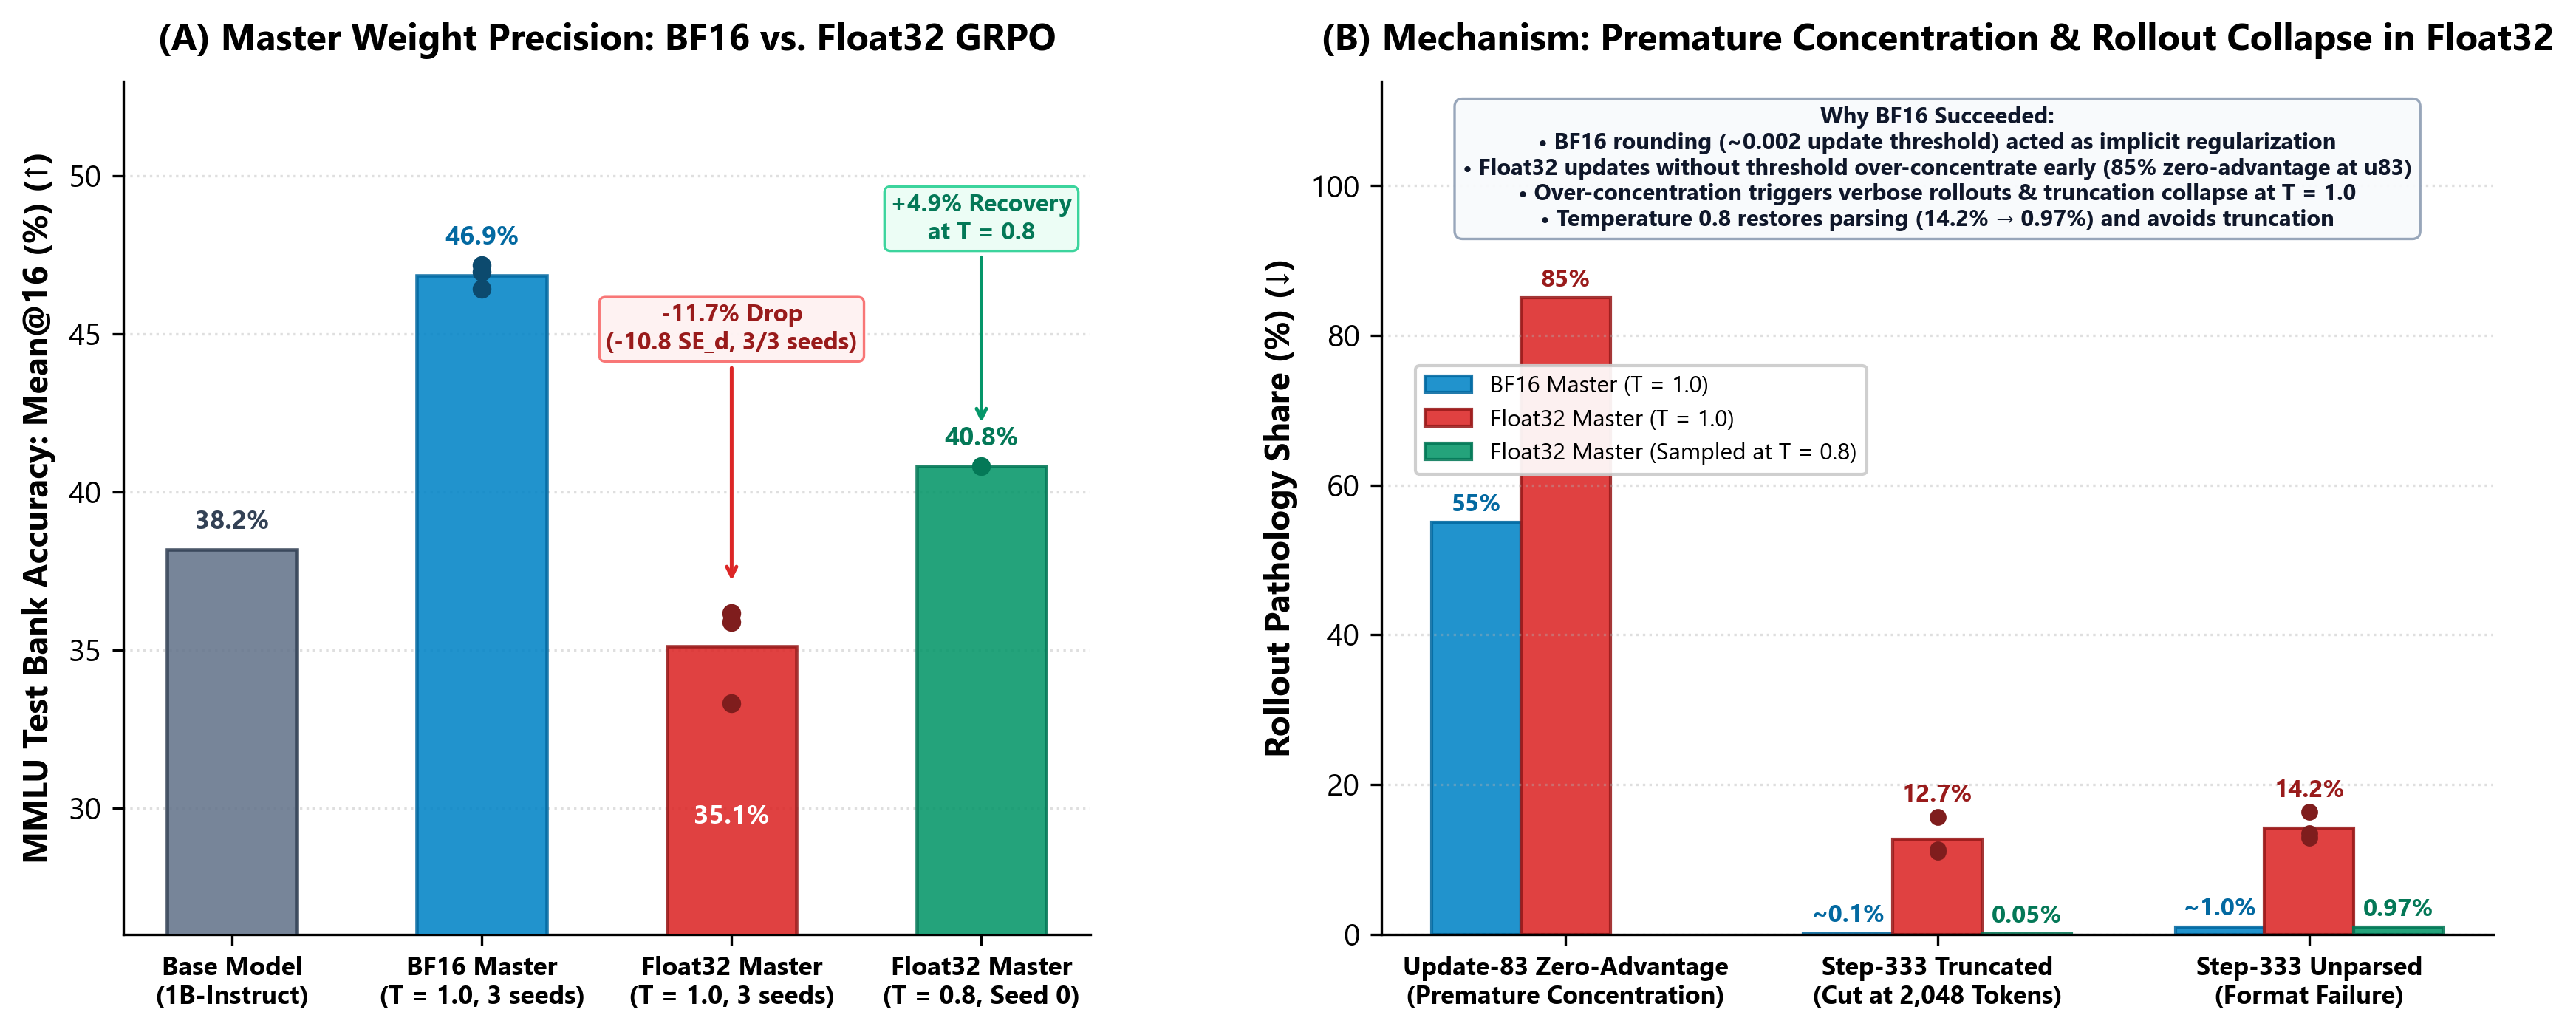
\includegraphics[height=0.51\textheight, keepaspectratio]{figures/talk_FigB2_fp32_vs_bf16_audit.png}
  \end{center}
  \vspace{-2.5mm}
  \begin{columns}[T, onlytextwidth]
    \begin{column}{0.485\textwidth}
      \psychbox{RedGRPO}{
        \textbf{\color{RedGRPO}1. Does \texttt{Float32} Break the $\sim 47\%$ RL Ceiling? No---It Collapses Early!}\\
        Testing whether \texttt{BF16} mantissa rounding ($\sim 0.002$ update threshold) caused the $\mathrm{Pass@1}$ ceiling reveals the exact opposite: removing rounding in \texttt{Float32} drops accuracy by $\mathbf{-11.7\%}$ ($46.9\% \to 35.1\%$, Panel A).
      }
    \end{column}
    \begin{column}{0.485\textwidth}
      \psychbox{BlueSFT}{
        \textbf{\color{BlueSFT}2. Psychometric Confirmation of Over-Sharpening}\\
        Without \texttt{BF16}'s implicit quantization floor, \texttt{Float32} updates over-concentrate prematurely ($\mathbf{85\%}$ dead zero-advantage rollouts by update 83 vs.\ $55\%$ in \texttt{BF16}, Panel B), triggering verbose truncation ($12.7\%$) and format failure ($14.2\%$).
      }
    \end{column}
  \end{columns}
\end{frame}

\end{document}
